%% 
%% Copyright 2007-2024 Elsevier Ltd
%% 
%% This file is part of the 'Elsarticle Bundle'.
%% ---------------------------------------------
%% 
%% It may be distributed under the conditions of the LaTeX Project Public
%% License, either version 1.3 of this license or (at your option) any
%% later version.  The latest version of this license is in
%%    http://www.latex-project.org/lppl.txt
%% and version 1.3 or later is part of all distributions of LaTeX
%% version 1999/12/01 or later.
%% 
%% The list of all files belonging to the 'Elsarticle Bundle' is
%% given in the file `manifest.txt'.
%% 
%% Template article for Elsevier's document class `elsarticle'
%% with numbered style bibliographic references
%% SP 2008/03/01
%% $Id: elsarticle-template-num.tex 249 2024-04-06 10:51:24Z rishi $
%%
\documentclass[preprint,12pt]{elsarticle}

%% Use the option review to obtain double line spacing
%% \documentclass[authoryear,preprint,review,12pt]{elsarticle}

%% Use the options 1p,twocolumn; 3p; 3p,twocolumn; 5p; or 5p,twocolumn
%% for a journal layout:
%% \documentclass[final,1p,times]{elsarticle}
%% \documentclass[final,1p,times,twocolumn]{elsarticle}
%% \documentclass[final,3p,times]{elsarticle}
%% \documentclass[final,3p,times,twocolumn]{elsarticle}
%% \documentclass[final,5p,times]{elsarticle}
%% \documentclass[final,5p,times,twocolumn]{elsarticle}

%% For including figures, graphicx.sty has been loaded in
%% elsarticle.cls. If you prefer to use the old commands
%% please give \usepackage{epsfig}

%% The amssymb package provides various useful mathematical symbols
\usepackage{amssymb}
%% The amsmath package provides various useful equation environments.
\usepackage{amsmath}
%% The amsthm package provides extended theorem environments
%% \usepackage{amsthm}

%% The lineno packages adds line numbers. Start line numbering with
%% \begin{linenumbers}, end it with \end{linenumbers}. Or switch it on
%% for the whole article with \linenumbers.
%% \usepackage{lineno}

\newcommand\hmmax{0}
\newcommand\bmmax{0}
\usepackage[T1]{fontenc} 
\usepackage[utf8]{inputenc}
\usepackage{amsmath}
\usepackage{amsthm}
\usepackage{amsfonts}
\usepackage{amssymb}
\usepackage{mathrsfs}
\usepackage{anyfontsize}
\usepackage{mdframed}
\usepackage{tikz}
\usepackage{verbatim}
\usepackage{booktabs}
\usepackage{array}
\usepackage{enumitem}
\usepackage{bbold}
\usepackage{fancyhdr}
\usepackage{blindtext}
\usepackage[top=1in, bottom=1.5in, left=1in, right=1in]{geometry}

\usepackage{MnSymbol}

\usepackage[cal=boondox,scr=boondoxo]{mathalfa}

\usepackage{float}
\usepackage{adjustbox}
\usepackage{subfig}
\usepackage{fancybox,graphicx}
\usepackage{caption}
\usepackage{color}
\usepackage{amsmath}  
\usepackage{stmaryrd}  
\usepackage{bm}  
\usepackage{bbm}
\usepackage{hyperref} % pour les liens hypertextes
\usepackage{cleveref}
\usepackage{setspace}

% DOI and ARXIV Commands for Bib Files
% Written by Daniel Herber
% -----------------------------------------------
% one option is to use the 'note' field with this command
% -----------------------------------------------
% for example, if your doi is 10.2514/1.J052182
% then for the citation for the reference in your bib file, use
% note = "\doi{10.2514/1.J052182}",
% -----------------------------------------------
% for example, if your arxiv number is 0706.1234
% then for the citation for the reference in your bib file, use
% note = "\arxiv{0706.1234}",

% requires hyperref package for \href command
\usepackage{hyperref}

% doi command (use in bib file)
\newcommand{\doi}[1]{{doi:~\href{https://doi.org/#1}{\nolinkurl{#1}}}\rmFullStop}

% arXiv command (use in bib file)
\newcommand{\arxiv}[1]{{arXiv:\href{https://arxiv.org/abs/#1}{#1}}\rmFullStop}

% command to remove full stop if the next character
\newcommand*{\rmFullStop}{\rmifnextchar{.}{}{}}

% command to check the next character and replace if present
% \rmifnextchar{X}{[removed text]}{[no X text]}
% if X is the next character, then it is removed and [removed text] is inserted
% otherwise, the character is not removed and [no X text] is inserted
% based on http://tex.stackexchange.com/questions/72827
\makeatletter
\newcommand{\rmifnextchar}[3]{%
  \begingroup
  \ltx@LocToksA{\endgroup#2}%
  \ltx@LocToksB{\endgroup#3}%
  \ltx@ifnextchar{#1}{%
    \def\next{\the\ltx@LocToksA}%
    \afterassignment\next
    \let\scratch= %
  }{%
    \the\ltx@LocToksB
  }%
}
\makeatother %doi command

\usepackage{accents}
\usepackage[titletoc,title]{appendix}


%floor and ceiling functions
\usepackage{mathtools}
\newcommand{\soft}{\mathcal{S}}
\newcommand{\hard}{\mathcal{H}}
\newcommand*\underdot[1]{ \underaccent{\bullet}{\mathcal{#1}} } %requiere: \usepackage{accents} 
\newcommand*\UnderDot[1]{ \underaccent{\bullet}{#1} } %requiere: \usepackage{accents} 

\usepackage{stackengine}
\newcommand\barbelow[1]{\stackunder[2.5pt]{$#1$}{\rule{1.2ex}{.15ex}}}

\newcommand{\pvec}[1]{\vec{#1}\mkern2mu\vphantom{#1}} %to prime a vector

\newcommand*\UnderTilde[1]{ \underaccent{\sim}{#1} }
  
\renewcommand{\figurename}{Fig.}
\journal{Nuclear Physics B}
\journal{Magnetic Resonance Imaging}

\newtheorem{theorem}{Proposition}
\renewcommand{\qedsymbol}{}
\newcommand{\parallelsum}{\mathbin{\!/\mkern-5mu/\!}}

\begin{document}

\title{Multiway multiblock logistic regression to classify liver tumors from MRI images} %% Article title

%% use optional labels to link authors explicitly to addresses:
%% \author[label1,label2]{}
%% \affiliation[label1]{organization={},
%%             addressline={},
%%             city={},
%%             postcode={},
%%             state={},
%%             country={}}
%%
%% \affiliation[label2]{organization={},
%%             addressline={},
%%             city={},
%%             postcode={},
%%             state={},
%%             country={}}

\author{Alexandre SELVESTREL} %% Author name

%% Author affiliation
\affiliation{organization={Université Paris-Saclay, CNRS, CentraleSupélec, Laboratoire des signaux et systèmes},%Department and Organization
            city={Gif-sur-Yvette},
            postcode={91190}, 
            country={France}}

            \begin{center}
              \vspace*{2cm}
              \setstretch{2} % Augmenter l'interligne
              {\LARGE \textbf{Rapport de stage de fin d'études sur l'analyse par machine learning de données médicales multivariées}} \\[7em]
              {\LARGE \textbf{Internship report on machine learning analysis of multivariate medical data}}\\[5em]
              {\large Alexandre SELVESTREL}\\[1em]
              {\large Laboratoire des systèmes, Centrale-Supélec}\\[1em]
              {\large Encadrants: Arthur Tenenhaus, Laurent Lebrusquet}\\
              \vspace*{\fill}
              Soutenance le 29 Novembre 2024
          \end{center}

\newpage
\newgeometry{top=2cm, bottom=2cm, left=1.5cm, right=1.5cm}
\noindent 
\begin{figure}[H]
    \centering
    
\includegraphics[scale = 0.85]{images/resume.pdf}
    \label{fig:odt_page}
\end{figure}

\newpage
\newgeometry{top=3cm, bottom=2cm, left=1.5cm, right=1.5cm}
\section*{Synthèse (version française)}
\vspace*{10 pt}
\paragraph*{Présentation générale} L'objectif de mon stage était de réaliser une classification automatique (via du machine learning) de tumeurs du foie basée sur des IRMs et sur quelques données cliniques (âge, sexe du patient ...). Cette classification devait permettre de tester et améliorer des modèles tensoriels récents \cite{multi_rank_1,multi_rank_r} et de vérifier si ceux-ci donnaient de meilleures performances que les autres modèles. Ce stage était effectué au laboratoire des systèmes (L2S) en partenariat avec l'assistance publique des hôpitaux de Paris (AP-HP). Sur le versan médical, nous avons pu bénéficier de l'aide de Sébastien Mulé, professeur à la faculté de santé, Université Paris-Est Créteil (UPEC) et Radiologie, chef du département imagerie de l'hôpital Henri Mondor.

\paragraph*{Enjeux} Ce stage s'inscrit dans la cadre de la collaboration entre le L2S et l'AP-HP. Du point de vue du L2S, il s'agit de mettre à l'épreuve des méthodes de machine learning particulières, basées sur des tenseurs et qui semblent spécifiquement adaptées aux données étudiées. Par ailleurs, en me formant au machine learning appliqué au domaine médical, le laboratoire s'assure qu'en poursuivant en doctorat, je disposerai des compétences nécessaires pour être immédiatement opérationnel.\\
\indent Pour l'AP-HP, l'enjeu est de faire progresser la recherche sur le cancer du foie. En effet, la détermination de la nature de la tumeur du foie d'un patient est un problème complexe auquel il n'existe pas de solution complètement satisfaisante à l'heure actuelle. Or, les médecins disposant des IRMs des patients malades, il serait dommage de ne pas les utiliser pour tenter de proposer un outil de diagnostic automatique. De plus, cet outil pourraît être utile aux médecins pour déterminer de nouveaux indicateurs qui caractérisent la classe d'une tumeur -en observant ce qui est considéré comme important par le modèle de classification automatique.

\paragraph*{Solutions et résultats:} Nous avons commencé par implémenter des modèles de machine learning basiques (régression logistique lasso et random forest) sur les données de cancer du foie. Cela nous a permis d'établir une valeur de référence pour la performance de la classification (AUC = 0.68). Nous avons ensuite cherché à améliorer ce score en développant une régression logistique tensorielle. Par ailleurs, nous avons proposé une variante de ce modèle tensoriel en intégrant la structure en blocs des données (section \ref{sec:models}). Ce nouveau modèle nous a permis de retrouver le score de départ, mais pas de l'améliorer.\\
\indent Afin de s'assurer de la pertinence de notre modèle, nous avons alors cherché à tester son efficacité sur des données simulées. Sur ces données, notre modèle tensoriel a montré des performances bien meilleures que les modèles non tensoriels, permettant même de mieux retrouver le coefficient de régression que d'autres modèles tensoriels déjà existant. Cela nous a permis de conclure que ce modèle était pertinent dans certains cas et que l'impossibilité d'améliorer les performances sur les données médicales était probablement due à la mauvaise qualité de ces données. Après plus d'un mois de travail pour améliorer la qualité des données, je me suis rendu à l'Hôpital Henri Mondor afin de parler de mes résultats avec Sébastien Mulé sur son lieu de travail (et non dans mon laboratoire comme les fois précédente). Cette visite a permis de découvrir l'existence d'un autre jeu de données, ommises jusqu'à présent, beaucoup plus simples (seulement une quinzaine de variables par individu), donnant des résultats bien meilleures que les données précédentes quand on les traite par machine learning (AUC = 0.95). Nous avons été surpris par l'arrivée au dernier moment de ces données qui, bien que de bonne qualité, ne sont pas adaptées aux modèles tensoriels. Nous ne les mentionnons donc pas dans la partie "article" du rapport mais nous les présentons juste après.\\

\newpage
\section*{Synthesis (english version)}
\vspace*{10 pt}

\paragraph*{Overview} The aim of my internship was to carry out an automatic classification (via machine learning) of liver tumors based on MRI scans and some clinical data (patient age, sex, etc.). The goal of this classification was to test and improve recent tensor models \cite{multi_rank_1,multi_rank_r} and check whether they performed better than other models. The internship was carried out at the systems laboratory (L2S), in partnership with the Assistance Publique des Hôpitaux de Paris (AP-HP). On the medical side, we benefited from the help of Sébastien Mulé, teacher at the Faculty of Health, Université Paris-Est Créteil (UPEC) and Radiology, Head of the Imaging Department at Henri Mondor Hospital.

\paragraph*{Stakes} This internship is part of the collaboration between L2S and AP-HP. From the point of view of the L2S, the aim is to put to the test particular machine learning methods, based on tensors, which seem specifically adapted to the data under study. What's more, by training me in machine learning applied to the medical field, the laboratory has ensured that if I go on to do a PhD, I will have the necessary skills to be immediately operational.\\
\indent For AP-HP, the challenge is to advance research into liver cancer. Determining the nature of a patient's liver tumor is a complex problem for which there is currently no completely satisfactory solution. Since doctors have access to MRI scans of patients with liver tumours, it would be a shame not to use them to try and offer an automatic diagnostic tool. In addition, this tool could be useful for radiologists to determine new indicators that characterize the class of a tumor - by observing what is considered important by the automatic classification model

\paragraph*{Solutions and results:} We started by implementing basic machine learning models (lasso logistic regression and random forest) on liver cancer data. This allowed us to establish a reference value for classification performance (AUC = 0.68). We then sought to improve this score by developing a tensor logistic regression. Furthermore, we proposed a variant of this tensor model by integrating the block structure of the data (section \ref{sec:models}). This new model allowed us to recover the initial score, but not to improve it.
\indent In order to ensure the relevance of our model, we then sought to test its effectiveness on simulated data. On this data, our tensor model showed much better performance than non-tensor models, even allowing us to find the regression coefficient better than other existing tensor models. This allowed us to conclude that this model was relevant in certain cases and that the impossibility of improving performance on medical data was probably due to the poor quality of this data. After more than a month of work to improve the quality of the data, I went to Henri Mondor Hospital to discuss my results with Sébastien Mulé at his workplace (and not in my laboratory as in previous times). This visit allowed me to discover the existence of another dataset, omitted until now, much simpler (only about fifteen variables per individual), giving much better results than the previous data when processed by machine learning (AUC = 0.95). We were surprised by the last-minute arrival of these data, which, although of good quality, are not suitable for tensor models. We therefore do not mention them in the "article" part of the report but present them just after.




\restoregeometry

\newpage
\tableofcontents
\newpage



\begin{frontmatter}

  
%% Title, authors and addresses

%% use the tnoteref command within \title for footnotes;
%% use the tnotetext command for theassociated footnote;
%% use the fnref command within \author or \affiliation for footnotes;
%% use the fntext command for theassociated footnote;
%% use the corref command within \author for corresponding author footnotes;
%% use the cortext command for theassociated footnote;
%% use the ead command for the email address,
%% and the form \ead[url] for the home page:
%% \title{Title\tnoteref{label1}}
%% \tnotetext[label1]{}
%% \author{Name\corref{cor1}\fnref{label2}}
%% \ead{email address}
%% \ead[url]{home page}
%% \fntext[label2]{}
%% \cortext[cor1]{}
%% \affiliation{organization={},
%%            addressline={}, 
%%            city={},
%%            postcode={}, 
%%            state={},
%%            country={}}
%% \fntext[label3]{}


%% Abstract
\begin{abstract}
    In this paper, we introduce a novel tensor logistic regression model designed for cases where the data is distributed across multiple tensors (referred to as blocs), each potentially having a different number of modes. We call this model Multiway Multibloc Logistic Regression (MMLR) and we also provide its fitting procedure. This model extends existing tensor logistic regressions \cite{multi_rank_1, multi_rank_r} to accommodate more complex data structures.
    This model is tested on simulated data and on real data (liver cancer MRI) in order to compare it to other models, tensor (multiway logistic regression \cite{multi_rank_r}) or non-tensor (lasso and group lasso \cite{grp_lasso}). The results of the MMLR are better than those of non-tensor models on simulated data and comparable to the state of the art on real data. In particular on simulated data, the regression coefficient is found more finely by the MMLR than by all the other models tested. 
    % is applied to the binary classification of liver tumors, distinguishing between hepatocellular carcinoma (HCC) and cholangiocarcinoma (CCK). This work extends the multiway logistic model presented in \cite{multi_rank_r} by organizing features into separate blocks. The dataset consists of liver MRI images acquired at four distinct time points (arterial, portal, venous, and delayed phases), supplemented by clinical variables. The performance of tensor models is evaluated in comparison with classical logistic regression and group lasso \cite{grp_lasso}, using both liver cancer data and simulated data.


\end{abstract}

% %%Graphical abstract
% \begin{graphicalabstract}
% %\includegraphics{grabs}
% \end{graphicalabstract}

% %%Research highlights
% \begin{highlights}
% \item Research highlight 1
% \item Research highlight 2
% \end{highlights}

%% Keywords
\begin{keyword}
  multiway data \sep multiblock data \sep MRI \sep tensor
%% keywords here, in the form: keyword \sep keyword

%% PACS codes here, in the form: \PACS code \sep code

%% MSC codes here, in the form: \MSC code \sep code
%% or \MSC[2008] code \sep code (2000 is the default)

\end{keyword}

\end{frontmatter}

%% Add \usepackage{lineno} before \begin{document} and uncomment 
%% following line to enable line numbers
%% \linenumbers

%% main text
%%

%% Use \section commands to start a section
\section{Introduction} 
% \noindent There are two main types of liver tumor: hepatocellular carcinoma (HCC) and cholangiocarcinoma (CCK). Some tumors even display both CCK and HCC characteristics, depending on the location of the liver observed, and are then said to be mixed. Since the treatment of liver tumors depends on their class, it is important to be able to distinguish them effectively. For the moment, there are two main approaches: microscopy and radiography with contrast injection.\\
% \indent Microscopy is the most reliable method, as it enables tumor cells to be analysed directly. However, since it requires the removal of a small piece of cancerous liver, it requires surgery and can lead to complications for the patient. What's more, it only gives access to a fragment of the liver, which is not necessarily representative of the tumor as a whole. Radiography (by MRI or scanner) with contrast injection, on the other hand, is non-invasive and give access to the entire 3D tumor. As the contrast medium diffuses into the liver, images are taken at four different times (arterial, portal, venous and late) to observe specific features of each phase. However, these images cannot be used to determine the nature of the tumor with the naked eye. Indeed, the characteristics of HCC and CCK tumors are often very similar, and experts do not always agree with each other when analyzing the images.\\
% \indent This article attempts to overcome the limitations of naked-eye analysis by using machine learning. Given the small number of patients studied (around $100$) and the requirement for explicability in the medical field, classical machine learning is preferred to deep learning. In addition, again because of the small number of patients and in order to simplify the study, mixed tumors are not taken into account. Indeed, these are still poorly understood by doctors, who sometimes even prefer to categorize them as HCC or CCK depending on which aspect predominates in the tumor.\\
% \indent The features of each tumor are extracted from the RMI images using the pyradiomics Python library \cite{pyradio}. For each patient, the tumor is observed on four separate images, taken at specific times corresponding to the different phases of acquisition (arterial, portal, venous and late). The same variables are therefore measured for each of these phases. Thus, for each patient, the features are organized according to a matrix of size $J \times K$ where $J$ is the number of features extracted by pyradiomics in each RMI image and $K$ is the number of acquisition phases. By stacking these matrices one on top of the other, for each individual, we form a tensor of size $n \times J \times K$, where $n$ is the number of individuals studied: we thus speak of tensorial data (Fig:\ref{fig:tensor}).\\
% \begin{figure}[tbp]
%     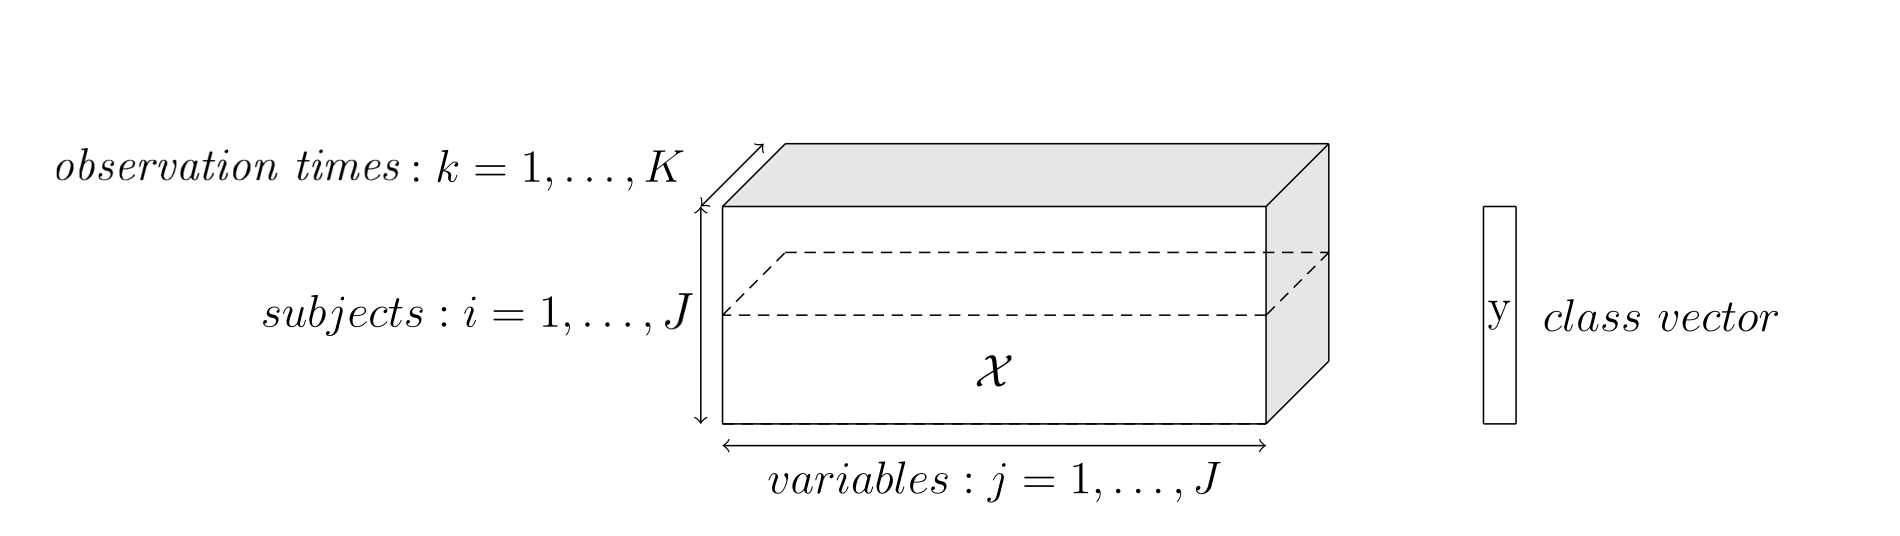
\includegraphics[width=0.9\textwidth]{images/tensor.png}
%     \caption{Example of order 3 tensor from \cite{multi_rank_r}}
%     \label{fig:tensor}
% \end{figure}
% \indent The model on which all the models presented in this article are based is lasso-penalized logistic regression. It allows parsimonious selection of explanatory variables, which is particularly useful when dealing with the large number of features extracted by pyradiomics. In order to take into account the tensorial structure of the data, several models specific to tensorial data, presented in section \ref{sec:models}, have been implemented.
% These models are based on the assumption that the tensor structure of the data should be reflected in the regression parameter $\bm{\beta}$ of the logistic regression \cite{multi_rank_1,multi_rank_r}. Thus, if the data forms a $3$-order tensor as shown in Fig \ref{fig:tensor}, we assume that $\bm{\beta}$ or at least a portion of $\bm{\beta}$ can be written as 
% \begin{equation}
% \sum\limits_{r = 1}^R \bm{\beta}_r^K \otimes  \bm{\beta}_r^J
% \end{equation}
% \noindent where "$\otimes $” is the kronecker product, $R$ is the maximum rank allowed for the considered portion of $\bm{\beta}$ and $\bm{\beta}_r^K$ and $\bm{\beta}_r^J$ are vectors.\\
% \indent These models are compared to the group lasso \cite{grp_lasso}, in order to check whether the simple grouping of variables into distinct packets can suffice to capture the relevant relationships between features (or whether it is essential to take full account of the tensor aspect of the data to obtain the best results). They are also compared to classical logistic regression. Furthermore, in order to assess the benefits of the models presented independently of medical data, their performance is first compared on simulated data. 


In many scientific fields, datasets are organized into multidimensional arrays that go beyond simple vectors or matrices. These arrays, called tensors, provide a natural way to represent data with multiple dimensions, also called in that case "modes". A tensor generalizes the concept of a matrix to higher dimensions: a vector is a tensor of order 1, a matrix is a tensor of order 2, and tensors of order 3 or more can encode relationships across three or more modes. 

To formalize this, consider a tensor \(\underline{\mathbf{X}} \in \mathbb{R}^{I \times J \times K}\) of order 3, where \(I\), \(J\), and \(K\) represent the dimensions along the three modes. Here, \(I\) might correspond to the number of individuals in a study, \(J\) to the number of observed variables, and \(K\) to the number of modalities or conditions under which these variables are measured. Each entry \(x_{ijk}\) in the tensor encodes the value of the \(j\)-th variable for the \(i\)-th individual under the \(k\)-th modality (see Fig. \ref{fig:tensor}). This structure allows the tensor to capture multi-dimensional relationships in a compact and meaningful way. For instance, while a matrix can describe how features vary across individuals, a tensor can extend this description to include variations across multiple modalities or acquisition phases. 

Tensors are particularly useful in applications where the relationships across modes are essential for understanding the data. For example, in medical imaging, radiomic features extracted from scans can be organized into tensors, where the modes might correspond to patients, extracted features, and different imaging phases. Preserving this structure enables models to exploit the inherent organization of the data, rather than flattening it into a less informative matrix.

Logistic regression, a classical tool for binary classification, has been extended to incorporate tensor data, allowing the regression parameters to reflect the multi-dimensional structure. These tensor logistic regression models have shown promise in leveraging the relationships across modes to improve both predictive accuracy and interpretability \cite{multi_rank_1, multi_rank_r}. However, existing methods often assume that the data can be represented as a single tensor,, which may not hold for more heterogeneous datasets. In this work, we propose the MMLR, an extension designed to handle datasets that naturally decompose into multiple tensors, each potentially with a different number of modes.

To evaluate the proposed approach, we test it on both simulated data and a real-world application in liver cancer classification. Liver tumors, which are among the most prevalent and deadly forms of cancer, are primarily classified into two types: hepatocellular carcinoma (HCC) and cholangiocarcinoma (CCK). Effective classification is crucial for determining appropriate treatment, but existing diagnostic methods face significant limitations. Microscopy, while reliable, is invasive and provides only a partial view of the tumor. Non-invasive radiographic imaging, such as MRI with contrast injection, captures a global view but is challenging to interpret due to overlapping characteristics of HCC and CCK. 

In this study, we represent liver tumors as third-order tensors constructed from radiomic features extracted from MRI scans. For each patient, four MRI images are acquired at different time points, corresponding to distinct phases of contrast enhancement: arterial, portal, venous, and late. These temporal phases capture specific characteristics of the tumor's vascularization, providing complementary information. The features extracted from each image are organized into a tensor with dimensions \( I \times J \times K \), where \( I \) is the number of patients, \( J \) is the number of features measured from each MRI image, and \( K = 4 \) corresponds to the four acquisition phases. This tensorial representation enables the application of our MMLR, which we compare against classical logistic regression, lasso-penalized logistic regression, and group lasso methods \cite{grp_lasso}.

This paper is organized as follows. In section \ref{sec:models}, we present tensor-based logistic regression models, starting with existing approaches and introducing the proposed MMLR. Then, section \ref{sec:simulated_data} and \ref{sec:real_data} describe the data used in this study, respectively simulated datasets and real-world MRI data from liver cancer patients. Finally, in section \ref{sec:results}, we detail the results of our experiments, comparing the performance of our model to state of the art methods on both types of data. 


\section{Methodology}

\subsection{Tensorial data and notations}

% We will denote as a tensor any multidimensionnal array, i.e. $\underline{\mathbf{X}} = (x_{i_1i_2...i_m})_{i_1 \in \llbracket 1, I_1 \rrbracket, i_2 \in \llbracket 1, I_2 \rrbracket, ... i_M \in \llbracket 1, I_M \rrbracket}$. It is the extension of the matrix to any finite dimension. To avoid confusion with the notion of dimension of a vector space, and in line with the conventions promoted in Kolda and Bader \cite{conventions}, these dimensons will be referred to as "mode" in the following and their number will be referred to as the "order" of the tensor.\\
\begin{figure}[tbp]
    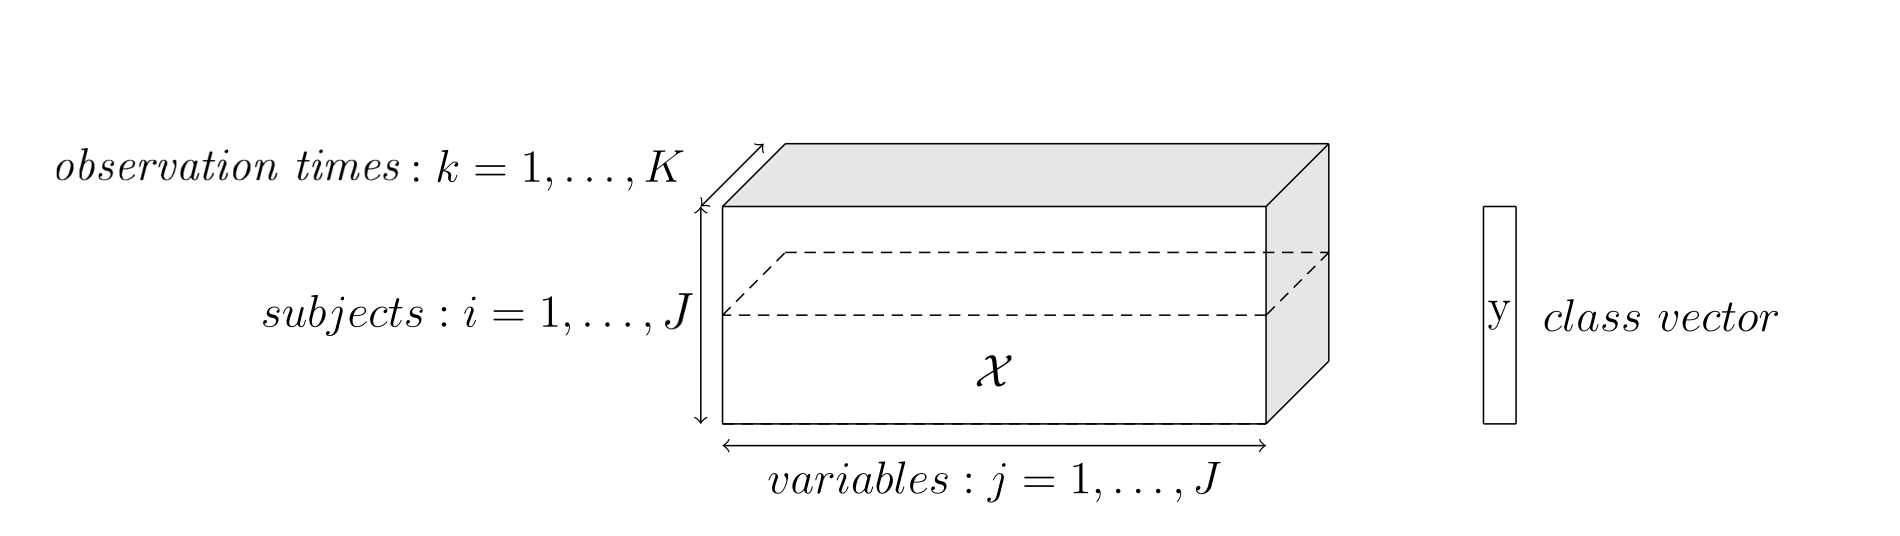
\includegraphics[width=0.9\textwidth]{images/tensor.png}
    \caption{Example of order 3 tensor from \cite{multi_rank_r}}
    \label{fig:tensor}
\end{figure}
\noindent We designate as tensor valued data any data where the explanatory variables are structured along several dimensions. To avoid confusion with the notion of dimension of a vector space we call these dimensions modes in the following. Then, instead of having a matrix of explanatory variables $\mathbf{X} = (x_{ij})_{i \in \llbracket 1, I \rrbracket, j \in \llbracket 1, J \rrbracket}$ (where $i$ is the individual and $j$ is the quantity of interest), we get a tensor of explanatory variables $\underline{\mathbf{X}} = (x_{ijk_1k_2\text{ ... }k_M})_{i \in \llbracket 1, I \rrbracket, j \in \llbracket 1, J \rrbracket, k_1 \in \llbracket 1, K_1 \rrbracket \text{ ... } k_m \in\llbracket 1, K_M \rrbracket } $  (where $i$ is the individual, $j$ is the quantity of interest and where for $m \in \llbracket 1, M \rrbracket$, $k_m$ is the $k_m$-th modality of the $m$-th mode of the data). We use the notations introduced in \cite{conventions}, especially concerning matricization (see section 2.4 of \cite{conventions}). For a self-contained document, we report some of them below.\\

\noindent $\bullet \; \;$ The concatenation of two matrices $\mathbf{A}$ and $\mathbf{B}$ by juxtaposing their columns side by side is denoted $[\mathbf{A} \; \; \mathbf{B}]$.\\
$\bullet \; \;$ To avoid overuse of the symbol $\phantom{a}^T$, we also define a notation to designate the juxtaposition of two matrices one below the other. Thus, the matrix defined by block with $\mathbf{A}$ above $\mathbf{B}$ is denoted $\left[\mathbf{A}; \, \mathbf{B}\right]$. It can also be written $[\mathbf{A}^T \; \; \mathbf{B}^T]^T$ but this multiplies the $\phantom{a}^T$ symbols, which impairs legibility. \\
$\bullet \; \;$ Since vectors are column matrices, using the same notation, we write the concatenation of two vectors $\mathbf{u}$ and $\mathbf{v}$ as follows: $[\mathbf{u}; \, \mathbf{v}]$.  \\
$\bullet \; \;$ The vector (column) whose elements are $(u_i)_{i \in \llbracket 1, I\rrbracket}$ is denoted $(u_1, u_2, \; \; \hdots \;\; u_I)$. \\
$\bullet \; \;$ If $\mathbf{X}$ is a matrix of explanatory variables, $\mathbf{x}_i$ is the vector (column) composed of the i-th row of $\mathbf{X}$.\\
$\bullet \; \;$ The vector of length $I$ filled with $1$ is denoted by $\mathbbm{1}_I$.\\
$\bullet \; \;$ We denote $\text{Diag}(\mathbf{u})$ the diagonal matrix whose diagonal is the vector $\mathbf{u}$. \\
$\bullet \; \;$ We denote $\mathbf{X}_{(1)}$ the transformation of a tensor $\underline{\mathbf{X}}$ into a matrix (by unfolding it) using the first mode to form the rows. This operation is called matricization. The order of the columns is lexicographic in the index of the modes. For a third order tensor, it gives $\mathbf{X}_{(1)} = [\mathbf{X}_{:\,:1} \; \; \ldots \; \;\mathbf{X}_{:\,:K}]$ 




\subsection{Machine learning models}
\label{sec:models}

\noindent In this section, we introduce the tensor models used in this article: the multiway logistic regression and the MMLR. For clarity and to avoid overcomplicating the notation, we focus on the case where $\underline{\mathbf{X}}$ is a third-order tensor, noting that the extension to higher-order tensors is straightforward. 
% We start briefly by non tensorial methods and then we describe in details the tensorial methods that we used. For the sake of simplicity, we only describe the situation where $\underline{\mathbf{X}}$ is a tensor of order 3. However, all the methods described here can be generalized to tensors of any order.
% \subsubsection{Non tensorial methods}
% For these methods, we start by unfolding the tensorial data $\underline{\mathbf{X}}$ into the matrix $\mathbf{X}_{(1)} = [\mathbf{X}_{:\,:1}\; \; \ldots \; \;\mathbf{X}_{:\,:K}]$. We then complete this matrix  by concatenating (along the columns) the matrix of non tensorial data $\mathbf{X}_{\text{tab}}$ (where "tab" stands for "tabular"). By doing so we obtain $\mathbf{X}_{\text{tot}} = [\mathbf{X}_{(1)} \; \; \mathbf{X}_{\text{tab}}]$.\\
% \indent We first train a penalized logistic regression lasso on $\mathbf{X}_{\text{tot}}$. Then, still based on the matrix $\mathbf{X}_{\text{tot}}$, we train a group lasso \cite{grp_lasso}. In order to make a comparison with tensorial models, we group by variable name or by mode. When the data is structure according to variable blocks, we finally group by block. 
\subsubsection{Multiway logistic regression}
\noindent We present the lasso penalized rank-R multiway logistic regression. This model is described in \cite{multi_rank_r}. The fundamental idea of the model is to decompose the parameter $\bm{\beta}_{\text{tens}} \in \mathbb{R}^{JK}$ associated with the tensor explanatory variables of the logistic regression as:
\begin{equation}
    \bm{\beta}_{\text{tens}} = \sum\limits_{r = 1}^R\bm{\beta}_r^K \otimes \bm{\beta}_r^J
\end{equation}
with for all $r \in \llbracket 1 ,R \rrbracket$, $\bm{\beta}_r^J \in \mathbb{R}^J$ and $\bm{\beta}_r^K \in \mathbb{R}^K$. To take account of the $M$ tabular variables (non tensorial), we associate them with a coefficient $\bm{\beta}_{\text{tab}} \in \mathbb{R}^M$. In this way, the parameter $\bm{\beta}$ of the logistic regression is written: $\left[\bm{\beta_{\text{tens}}}; \, \bm{\beta_{\text{tab}}} \right]$.\\
As usual with logistic regressions, we consider that each realization of the explained variable $y_i$ ($i \in \llbracket 1, I \rrbracket$) follows an independent Bernoulli law conditionally on $\mathbf{x_i}$. For logistic regression, this probability is parametrzied by $\bm{\beta}$ and defined as
\begin{equation}
    \label{eqref:vraisemblance}
    \mathbb{P}( y_i = 1\, | \, \mathbf{x}_i) = \frac{1}{1 + \exp(- \mathbf{x}_i^T \bm{\beta} - \beta_0)}
\end{equation}
where  $\beta_0 \in \mathbb{R}$ is the intercept.\\ %and $\mathbf{x}_i \in \mathbb{R}^{JK}$ is given by $\mathbf{x}_i = {(\mathbf{x}_{\text{tot}}})_{i:}$ \\

\noindent We set  $\bm{\beta}^J = \left[\bm{\beta}_1^J ; \;\; \hdots \; \; ;\,\bm{\beta}_R^J \right]$ and  $\bm{\beta}^K = \left[\bm{\beta}_1^K; \; \; \hdots \; \; ;\,\bm{\beta}_R^K \right]$.
\vspace{5 pt}
\noindent in order to promote sparsity, we add L1 type penalties. It yields to consider the following optimization problem: %\in \mathbb{R}\times \mathbb{R}^{RJ} \times  \mathbb{R}^{RK} \times \mathbb{R}^M
\begin{equation}
    \beta_0, \bm{\beta}^J, \bm{\beta}^K, \bm{\beta}_{\text{tab}} \; = \hspace{-8pt} \underset{\beta_0 ,\, \bm{\beta}^J, \, \bm{\beta}^K, \, \bm{\beta}_{\text{tab}}}{\text{argmin}} \left[ - \sum\limits_{i = 1}^{I} \log(\mathbb{P}(y_i = 1 \, | \mathbf{x}_i)) + \lambda \left(\sum\limits_{r = 1}^R
    \lVert \bm{\beta}_r^K \otimes \bm{\beta}_r^J \rVert_1 + \lVert \bm{\beta}_{\text{tab}} \rVert_1 \right)\right]
\end{equation}

\noindent Optimization is performed by alternating directions between $\left[ \beta_0 ;\, \bm{\beta}^J  ; \,  \bm{\beta}_{\text{tab}}   \right]$ and  $\left[ \beta_0; \, \bm{\beta}^K  ;\, \bm{\beta}_{\text{tab}}  \right]$.  We note that optimizing the loss function in each of these directions boils down to perform a simple logistic regression with a lasso penalty. Indeed, if we denote $C$ the loss function of classical logistic regression penalized by lasso (for any $K_0 \in \mathbb{N}^{*}$):

% The stopping criterion is defined by the relative difference between the value of the objective function before optimization in the first direction and the value of the same function after optimization in the second direction.

\begin{equation}
    %% Gerer l'allign
    C: \begin{cases}
        \begin{array}{ccl}
            \mathbb{R} \times \mathbb{R}^{K_0} \times \mathbb{R}^{I \times K_0} \times \mathbb{R}^{I} \times \mathbb{R} & \longrightarrow & \mathbb{R}                                                                                                                                                                    \\
            (\beta_0, \bm{\beta}, \mathbf{X}, \mathbf{y}, \lambda )                                                     & \longmapsto     & -\displaystyle{\sum\limits_{i = 1}^I} [ y_i(\beta_0 + \mathbf{x}_i^T \bm{\beta}) - \log(1 + \exp(\beta_0 + \mathbf{x}_i^T \bm{\beta})) ] + \lambda \lVert \bm{\beta} \rVert_1
        \end{array}
    \end{cases}
\end{equation}

\noindent optimizing the overall loss function with respect to $\left[ \beta_0;\, \bm{\beta}^J ;\, \bm{\beta}_{\text{uni}}  \right]$ is equivalent to solve
\begin{equation}
    \underset{(\beta_0, \bm{\beta}) \in \mathbb{R} \times \mathbb{R}^{JR + M}}{\text{argmin}}  C(\beta_0, (\mathbf{Q}^J)^{-1}\bm{\beta},\mathbf{Z}^J \mathbf{Q}^J, \mathbf{y}, \lambda)
\end{equation}
\noindent Where $\mathbf{Q}^J$ and $\mathbf{Z}^J$ are defined as follows:
\begin{align}
    \mathbf{Z}^J                                                                               & = [\mathbf{Z}_1^J \; \; \hdots \; \; \mathbf{Z}_R^J \; \;  \mathbf{X}_{\text{tab}}]                                                                             \\
    \text{where} \; \forall r \in \llbracket 1, R\rrbracket\, , \hspace{0.5 cm} \mathbf{Z_r^J} & = \sum\limits_{k = 1}^K (\beta_r^K)_k  \, \mathbf{X}_{::k} \hspace{0.5 cm} (\mathbf{Z}_r^J \in \mathbb{R}^{N \times J})                                             \\
    \hspace{7 pt}
    \text{and} \hspace{0.5 cm} \mathbf{Q}^J & = \text{Diag}([\lVert \bm{\beta}_1^K \rVert_1^{-1} \mathbbm{1}_J; \; \; \hdots \; \; ;\, \lVert \bm{\beta}_R^K \rVert_1^{-1} \mathbbm{1}_J ;\,  \mathbbm{1}_M])
\end{align}
\hspace{10 pt}
\noindent Girka et al. \cite{multi_rank_r} demonstrate this result by noting that for $i \in \llbracket 1, I\rrbracket$,

\begin{align}
    {{\mathbf{x}_{(1)}}_i}^{\hspace{-5 pt} T} \left( \sum\limits_{r = 1}^R \bm{\beta}_r^K \otimes \bm{\beta}_r^J \right) & = \sum\limits_{r = 1}^R \left[({{\mathbf{x}_{(1)}}_i}^{\hspace{-5 pt} T}   \left( \bm{\beta}_r^K  \otimes \mathbf{I}_J\right)\right] \bm{\beta}_r^J \\
                                                                                                                         & = \sum\limits_{r = 1}^R (\mathbf{z}_r^J)_i^T \bm{\beta}_r^J
\end{align}

\noindent and that

\begin{align}
                                & \sum\limits_{r = 1}^R \lVert \bm{\beta}_r^K \otimes \bm{\beta}_r^J \rVert_1 = \lVert \mathbf{R}_{\text{tens}}^J \bm{\beta}^J\rVert_1                             \\
    \text{with} \hspace{0.5 cm} & \mathbf{R}_{\text{tens}}^J = \text{Diag}([\lVert \bm{\beta}_1^K \rVert_1 \mathbbm{1}_J; \; \; \hdots \; \; ; \,  \lVert \bm{\beta}_R^K \rVert_1 \mathbbm{1}_J ])
\end{align}

\noindent Thus,
\begin{align}
                               & (\mathbf{x}_{\text{tot}})_i^T \bm{\beta}= (\mathbf{z}_i^J)^T [\bm{\beta}^J; \bm{\beta}_{\text{tab}}] \\
    \text{and} \hspace{0.5 cm} & \sum\limits_{i = 1}^I
    \lVert \bm{\beta}_r^K \otimes \bm{\beta}_r^J \rVert_1 + \lVert \bm{\beta}_{\text{tab}} \rVert_1= \lVert (\mathbf{Q}^J)^{-1} \bm{\beta} \rVert_1
\end{align}
This justifies the previous results\\[5 pt]
\noindent For optimization with respect to $\left[ \beta_0; \, \bm{\beta}^K; \, \bm{\beta}_{\text{tab}}  \right]$ , the method follows the same steps. The only difference concerns the definition of $\mathbf{Z}^K$. It is:
\begin{align}
                                                                         & \mathbf{Z}^K = [\mathbf{Z}_1^K \; \; \hdots \; \; \mathbf{Z}_R^K \; \; \mathbf{X}_{\text{tab}}] \\
    \text{with} \forall r \in \llbracket 1, R \rrbracket \hspace{0.5 cm} & \mathbf{Z}_r^K = \sum\limits_{j = 1}^J (\beta_r^J)_j \mathbf{X}_{:j:}
\end{align}

\noindent This is justified by:

\begin{align}
    {{\mathbf{x}_{(1)}}_i}^{\hspace{-5 pt} T}  \left( \sum\limits_{r = 1}^R \bm{\beta}_r^K \otimes \bm{\beta}_r^J \right) & = \sum\limits_{r = 1}^R \left[ ({{\mathbf{x}_{(1)}}_i}^{\hspace{-5 pt} T}  \left( I_K \otimes \bm{\beta}_r^J \right) \right] \bm{\beta}_r^K \\
                                                                                                                          & = \sum\limits_{r = 1}^R (\mathbf{z}_r^K)_i^T \bm{\beta}_r^K
\end{align}

\subsubsection{Multiway and Multibloc Logistic Regression (MMLR)}

\noindent This section presents lasso penalized MMLR. This model draws heavily on the multiway logistic regression we have just presented, while also taking into account a block structure of tensor data. More precisely, each of these blocks $\underline{\mathbf{X}}^{l}$  is a tensor and has its own independent coefficient $\bm{\beta}_l \,$. We also allow each block to have its own rank $R_l$. As tabular quantities are not measured according to several modalities, they are not placed in any particular block. They will be included in the model in the same way as in the multiway case. Mathematically, we define the model as follows:\\
\indent Let $L \in \mathbb{N}^{*}$ denote the number of blocks. For any $l \in \llbracket 1, L \rrbracket$, let $J_l$ be the number of tensorial variables in block $l$. The matrix of explanatory variables is defined by $\mathbf{X}^{'} = [\mathbf{X}^1_{(1)} \; \hdots \; \; \mathbf{X}^L_{(1)}] $ and $\bm{\beta}$ is the regression coefficient with respect to this matrix. The new $\bm{\beta}$ structure is given by blocks. It is:
\begin{equation}
    \bm{\beta} = \left[ \sum\limits_{r = 1}^{R_1} \bm{\beta}_{(1,r)}^K \otimes \bm{\beta}_{(1,r)}^J;   \; \; \hdots  \; \; ;\, \sum\limits_{r = 1}^{R_L}\bm{\beta}_{(L,r)}^K \otimes \bm{\beta}_{(L,r)}^J\; ;\,\bm{\beta}_{\text{tab}}   \right]
\end{equation}
With for all $l \in \llbracket 1,L \rrbracket$ , we have $r \in \llbracket 1, R_l\rrbracket$,  $\bm{\beta}_{(l,r)}^J \in \mathbb{R}^{J_l}$ and $\bm{\beta}_{(l,r)}^K \in \mathbb{R}^{K}$. \\

\noindent We call $\bm{\beta}^J$ and $\bm{\beta}^K$ the vectors
\begin{align}
    \bm{\beta}^J & = \left[ \bm{\beta}_{(1,1)}^J\, ; \hspace{7 pt} \hdots \hspace{7 pt} \, ; \, \bm{\beta}_{(1,R_1)}^J \,;    \hspace{7 pt} \hdots \hspace{7 pt}  \hdots \hspace{7 pt} \, ; \,  \bm{\beta}_{(L,1)}^J   \hspace{7 pt} \hdots \hspace{7 pt}  \, ;\,\bm{\beta}_{(L,R_L)}^J   \right] \\
    \bm{\beta}^K & = \left[ \bm{\beta}_{(1,1)}^K\, ; \hspace{7 pt} \hdots \hspace{7 pt} \, ; \, \bm{\beta}_{(1,R_1)}^K \,;    \hspace{7 pt} \hdots \hspace{7 pt}  \hdots \hspace{7 pt} \, ; \,  \bm{\beta}_{(L,1)}^K   \hspace{7 pt} \hdots \hspace{7 pt}  \, ;\,\bm{\beta}_{(L,R_L)}^K   \right]
\end{align}
% Indiquer qui est l et r après et changer les beta montrés (cf cahier)

\noindent In a similar way to what is done in the multiway model, we adapt the lasso penalty, so that the new optimization problem becomes:
\begin{equation}
    \beta_0 ,\, \bm{\beta}^J, \, \bm{\beta}^K, \, \bm{\beta}_{\text{tab}} = \hspace{- 8 pt} \underset{\beta_0 ,\, \bm{\beta}^J, \, \bm{\beta}^K, \, \bm{\beta}_{\text{tab}}}{\text{argmin}} \left(  - \sum\limits_{i = 1}^{I} \log(\mathbb{P}(y_i = 1 \, | \mathbf{x}_i)) + \sum\limits_{l = 1}^L \sum\limits_{r = 1}^{R_l}
    \lVert \bm{\beta}_{(l,r)}^K \otimes \bm{\beta}_{(l,r)}^J \rVert_1 + \lVert \bm{\beta}_{\text{tab}} \rVert_1 \right)
\end{equation}

\noindent Once again, this problem is solved by alternating optimization directions $\left[ \beta_0 ;\, \bm{\beta}^J ;\,  \bm{\beta}_{\text{tab}} \right]$ and\\
$\left[ \beta_0 ;\, \bm{\beta}^K ;\,  \bm{\beta}_{\text{tab}} \right]$. Each of these two problems can be reduced to a lasso-penalized classical logistic regression\\[3 pt]
Indeed, optimizing according to $\left[ \beta_0 ;\, \bm{\beta}^J ;\,  \bm{\beta}_{\text{tab}} \right]$ is equivalent to searching
\begin{equation}
    \underset{(\beta_0, \bm{\beta}) }{\text{argmin} \;}  C(\beta_0, (\mathbf{Q}^J)^{-1}\bm{\beta},\mathbf{Z}^J \mathbf{Q}^J, \mathbf{y}, \lambda)
\end{equation}
Where $\mathbf{Q}^J$ and $\mathbf{Z}^J$ are defined as follows:

\begin{align}
    \mathbf{Z}^J = [ \mathbf{Z}_{(1,1)}^J \; \; \hdots \; \;                                                        & \mathbf{Z}_{(1,R_1)}^J  \; \; \hdots  \; \; \hdots \; \; \mathbf{Z}_{(L,1)}^J \; \; \hdots \; \; \mathbf{Z}_{(L,R_L)}^J \; \; \mathbf{X}_{\text{tab}}] \label{eqref: Z_j}                                                                                                                      \\
    \text{where} \; \forall r \in \llbracket 1, R_l\rrbracket\, , \hspace{0.5 cm} \mathbf{Z}_{(l,r)}^J                & = \sum\limits_{k = 1}^K \left(\beta_{(l,r)}^K\right)_k\mathbf{X}^l_{::k}  \hspace{0.5 cm} \left(\mathbf{Z}_{(l,r)}^J \in \mathbb{R}^{I \times J_l}\right) \label{eqref: Z_r}                                                                                                               \\
    \hspace{7 pt}
    \mathbf{Q}^J = \text{Diag}([\lVert \bm{\beta}_{(1,1)}^K \rVert_1^{-1} \mathbbm{1}_{d_1}; \; \; \hdots \; \;; \, & \lVert \bm{\beta}_{(1,R_1)}^K \rVert_1^{-1} \mathbbm{1}_{d_1};  \; \; \hdots \; \;  \hdots \; \; ;\, \lVert \bm{\beta}_{(L,1)}^K \rVert_1^{-1} \mathbbm{1}_{J_L};  \; \;  \hdots \; \; ;\, \lVert \bm{\beta}_{(L,R_L)}^K \rVert_1^{-1} \mathbbm{1}_{J_L}; \, \mathbbm{1}_M]) \label{eqref:Q^J}
\end{align}

The demonstration of this result is similar to that of the multiway case. Indeed, we note that
\begin{align}
    \hspace{-40 pt}(\mathbf{x}')_i^T \left[ \sum\limits_{r = 1}^{R_1} \bm{\beta}_{(1,r)}^K \otimes \bm{\beta}_{(1,r)}^J;   \; \; \hdots  \; \; ;\, \sum\limits_{r = 1}^{R_L} \bm{\beta}_{(L,r)}^K \otimes \bm{\beta}_{(L,r)}^J \right] & = \sum\limits_{l = 1}^L \sum\limits_{r = 1}^{R_l} \left(\mathbf{x}^l\right)_i^T \left(\bm{\beta}_{(l,r)}^K \otimes \bm{\beta}_{(l,r)}^J \right)                        \\
                                                                                                                                                                                                                                     & = \sum\limits_{l = 1}^L \sum\limits_{r = 1}^{R_l} \left[ \left(\mathbf{x}^l\right)_i^T \left( \bm{\beta}_{(l,r)}^K \otimes I_{J_l} \right) \right]\bm{\beta}_{(l,r)}^J \\
                                                                                                                                                                                                                                     & = \sum\limits_{l = 1}^L \sum\limits_{r = 1}^{R_l}\left(\mathbf{z}_{(l,r)}^J\right)_i^T \bm{\beta}_{(l,r)}^J
\end{align}

And that

\begin{align}
    \sum\limits_{l = 1}^L \sum\limits_{r = 1}^{R_l} \lVert \bm{\beta}_{(l,r)}^K \otimes \bm{\beta}_{(l,r)}^J \rVert_1                                            & = \lVert \mathbf{R}_{\text{tens}}^J \bm{\beta}^J\rVert_1                                                                                                                                                                                                  \\
    \text{with} \hspace{0.5 cm} \mathbf{R}_{\text{tens}}^J = \text{Diag}    ([\lVert \bm{\beta}_{(1,1)}^K \rVert_1 \mathbbm{1}_{d_1}; \; \; \hdots \; \;; \, & \lVert \bm{\beta}_{(1,R_1)}^K \rVert_1 \mathbbm{1}_{d_1};  \; \; \hdots \; \;  \hdots \; \; ;\, \lVert \bm{\beta}_{(L,1)}^K \rVert_1 \mathbbm{1}_{J_L};  \; \;  \hdots \; \; ;\, \lVert \bm{\beta}_{(L,R_L)}^K \rVert_1 \mathbbm{1}_{J_L}; \, \mathbbm{1}_M])
\end{align}

\noindent We deduce that

\begin{align}
                               & [{\mathbf{x}'}_i; \, \mathbf{x}_{\text{tab}\raisebox{-4pt}{$\scriptstyle i$}}]\, \bm{\beta}= (\mathbf{z}_i^J)^T [\bm{\beta}^J; \, \bm{\beta}_{\text{tab}}]                                 \\
    \text{and} \hspace{0.5 cm} & \sum\limits_{l = 1}^L \sum\limits_{r = 1}^{R_l} \lVert \bm{\beta}_{(l,r)}^K \otimes \bm{\beta}_{(l,r)}^J \rVert_1 + \lVert \bm{\beta}_{\text{uni}} \rVert_1= \lVert (\mathbf{Q}^J)^{-1} \bm{\beta} \rVert_1
\end{align}

\noindent Wich justifies the previous results.\\[5 pt]
\noindent For optimization with respect to $\left[ \beta_0 ;\, \bm{\beta}^K ;\,  \bm{\beta}_{\text{tab}} \right]$, the method is similar. The only difference concerns the form of $\mathbf{Z}^K$. It is written as:
\begin{align}
    \mathbf{Z}^K	=[ \mathbf{Z}_{(1,1)}^K \; \; \hdots \; \;                                          & \mathbf{Z}_{(1,R_1)}^K  \; \; \hdots  \; \; \hdots \; \; \mathbf{Z}_{(L,1)}^K \; \; \hdots \; \; \mathbf{Z}_{(L,R_L)}^K \; \; \mathbf{X}_{\text{tab}}] \label{eqref: Z^K}               \\
    \text{where} \; \forall r \in \llbracket 1, R_l\rrbracket\, , \hspace{0.5 cm} \mathbf{Z}_{(l,r)}^K & = \sum\limits_{j = 1}^{J_l} \mathbf{X}_{:j:}^l \left(\beta_{(l,r)}^J\right)_j \hspace{0.5 cm} \left(\mathbf{Z}_{(l,r)}^K \in \mathbb{R}^{I \times K}\right) \label{eqref: Z_tens^K}
\end{align}

\noindent The justification of that last result is analogous to the one used in the multiway case.\\[10 pt]
In order to clarify the algorithm that we use, we give here the pseudo-code of our implementation\\[5 pt]

{\fontsize{12}{8}\selectfont \noindent \textbf{Fitting algorithm for MMLR:}}\\[1 pt]
\begin{mdframed}[leftmargin=0cm, rightmargin=0.2cm]
    \noindent \textbf{Inputs}\\
    \phantom{a}\hspace{5 pt} $\bullet$ $\epsilon >0$, $\lambda >0$, $R \in \mathbb{N}^{*}$\\[2 pt]
    \phantom{a}\hspace{5 pt} $\bullet$ $\bm{\beta}^{K(0)} \in \mathbb{R}^{LRK}$\\[4 pt]
    \textbf{Treatment}\\
    \phantom{a}\hspace{5 pt} $\bullet$ $q \leftarrow 0$\\[2 pt]
    \phantom{a}\hspace{5 pt}  \textbf{Repeat}\\[2 pt]
    \begin{tikzpicture}[overlay, remember picture]
        \draw[thick] (0.9, 0.18) -- (0.9, -4.25);  % Modifier les coordonnées pour ajuster la position et la
    \end{tikzpicture}
    \phantom{a}\hspace{22 pt} $\bullet$ Construct $\mathbf{Z}^J$ according to \cref{eqref: Z_j,eqref: Z_r}\\[2 pt]
    \phantom{a}\hspace{25 pt} $\bullet$ Construct $\mathbf{Q}^J$ according to \cref{eqref:Q^J}\\[2 pt]
    \phantom{a}\hspace{25 pt}  $\bullet$ $(\beta_0^{J {(q)}}, \bm{\beta}^{J {(q)}}) \longleftarrow \hspace{-10 pt} \underset{(\beta_0, \bm{\beta}) \in \mathbb{R} \times \mathbb{R}^{RJ + M}}{\text{argmin}} \left( C(\beta_0, (\mathbf{Q}^J)^{-1}\bm{\beta},\mathbf{Z}^J \mathbf{Q}^J, \mathbf{y}, \lambda) \right)$\\[2 pt]
    \phantom{a}\hspace{25 pt} $\bullet$ Construct $\mathbf{Z}^K$ according to \cref{eqref: Z^K,eqref: Z_tens^K}\\[3 pt]
    \phantom{a}\hspace{25 pt} $\bullet$ Construct $\mathbf{Q}^K$ by adapting \cref{eqref:Q^J}\\[2 pt]
    \phantom{a}\hspace{25 pt}  $\bullet$ $(\beta_0^{K {(q)}}, \bm{\beta}^{K {(q)}}) \longleftarrow \hspace{-10 pt} \underset{(\beta_0, \bm{\beta}) \in \mathbb{R} \times \mathbb{R}^{LRK + M}}{\text{argmin}} \left( C(\beta_0, (\mathbf{Q}^K)^{-1}\bm{\beta},\mathbf{Z}^K \mathbf{Q}^K, \mathbf{y}, \lambda) \right)$\\[2 pt]
    \phantom{a}\hspace{25 pt}  $\bullet$ $q \leftarrow q + 1$\\[4 pt]
    \phantom{a}\hspace{8 pt}  \textbf{until} $|C^K - C^J| < \epsilon |C^J| $ \; (where $C^K$ and $C^J$ are respectively\\[2 pt]
    \phantom{a}\hspace{42 pt} $C(\beta_0^{J {(q)}}, (\mathbf{Q}^J)^{-1}\bm{\beta}^{J {(q)}},\mathbf{Z}^J \mathbf{Q}^J, \mathbf{y}, \lambda)$) and $C(\beta_0^{K {(q)}}, (\mathbf{Q}^K)^{-1}\bm{\beta}^{K {(q)}},\mathbf{Z}^K \mathbf{Q}^K, \mathbf{y}, \lambda)$)\\ [8 pt]
    \textbf{Return} $(\beta_0^{K {(q)}},\bm{\beta}^{K(q)}, \bm{\beta}^{J(q)})$
\end{mdframed}

\vspace{5 pt}
\noindent \textbf{Notes}:
\begin{itemize}
    \item The worst-case complexity of the tensor algorithms presented here is $O(J + K + R)$, compared with $O(JK)$ for non-tensor algorithms. So, if $J$ and $K$ are large and supposing $R \ll \min(J,K)$ then tensor algorithms are more efficient, as shown in \cite{multi_rank_r}.
    \item With the multiway multiblock model, we can deal with the case where each block is a tensor of different order. All we need to do is optimize several times according to the same $\bm{\beta}$ mode in blocks with fewer modes than the others.
    \item We decided to optimize the loss function completely in one direction before turning to the other one instead of alternating one step in each direction because the first procedure was more stable and could be implemented efficiently using the glmnet package in R \cite{glmnet}.
\end{itemize}

\vspace{7 pt}


\subsection{Simulated data generation}
\label{sec:simulated_data}
\noindent To test the MMLR, we perform tests on simulated data. In this section, we explain how we generate this data.
\subsubsection{Regression parameter structure}

\noindent In order, to mimic the structure of real multiblock tensor data, we have organized our simulated data into several tensors (i.e. blocks). This enables us to compare the performance of the MMLR with other logistic models.\\
\indent The multiway and multiblock aspect of the MMLR is reflected in its regression parameter $\bm{\beta}$. This is why we have chosen to generate our data in such a way that the optimal regression parameter $\bm{\beta}^*$ (i.e. minimizing the classification error) has a multiblock multiway structure. To make the reconstruction of the regression parameter as visual as possible, we reused the pictograms presented in \cite{picto}. A modified version of these pictograms is presented in Fig \ref{fig:fourchette} $\&$ \ref{fig:picto_blocs}. Thus, $\bm{\beta}^*$ is in fact composed exclusively of $0$ and $1$. The $1$ are arranged to form simple geometric patterns when the beta vector is split into several lines (Fig: \ref{fig:fourchette}). The result is $\bm{\beta}^*$ in the form of a second-order tensor, each column of which is associated with a different explanatory variable and each row with a different observation modality. As pictograms are simple, the rank of the tensor is expected to be low in relation to the number of variables and modalities.\\
\indent To add a multiblock aspect to $\bm{\beta}^*$, instead of choosing just one pictogram, we consider the column-wise concatenation of several pictograms (Fig: \ref{fig:picto_blocs}). Thus, each pictogram, seen as a 2nd-order tensor, is of low rank, but the concatenation of several pictograms produces a tensor of higher rank. It is this concatenation which, after being unfolded into a single line, constitutes $\bm{\beta}^*$. This renders the single multiway logistic regression model less relevant (which will need to have a high rank to correctly reconstruct $\bm{\beta}^*$), without putting the multiway multiblock model at a disadvantage (which will be able to separate $\bm{\beta}^*$ into several tensors of lower rank: one per pictogram).


\begin{figure}[tbp]
    \centering
    \begin{minipage}{0.45\textwidth}
        \centering
        
\includegraphics[scale = 0.2]{./images/fourchette.png}
        \caption{Example of the pictogram used to generate $\bm{\beta}$.}
        \label{fig:fourchette}
    \end{minipage}
    \hfill
    \begin{minipage}{0.45\textwidth}
        \centering
        
\includegraphics[scale = 0.2]{./images/3_picto.png}
        \caption{Example of pictogram concatenation used to generate $\bm{\beta$}.}
        \label{fig:picto_blocs}
    \end{minipage}
\end{figure}

\subsubsection{Generation of explanatory variables}
The method generally used to simulate explanatory variables in regression models is to use a simple probability distribution (often the standardized normal distribution), identical for all individuals. The explained variable is then obtained by applying the regression model with $\bm{\beta} = \bm{\beta}^*$ to the explanatory variables. This is, for example, what is proposed in \cite{picto}. However, this method poses a problem in binary classification, as we have no control over the number of individuals in each class.\\
\indent To overcome this difficulty, we decided to generate the explanatory variables differently. For each individual class, we chose to generate the explanatory variables according to a multivariate normal distribution. The two classes have the same covariance matrix, but different means. These means and covariance matrices are chosen to ensure that $\bm{\beta}^*$ is indeed the normal vector to the best class-separation hyperplane. To prove this, we will demonstrate that the method used ensures that this hyperplane is the Bayes classifier minimizing the classification error for the simulated data.\\
\begin{theorem}
Noting respectively $\bm{\mu}_0$ and $\bm{\mu}_1$ the mean vectors of the $J$ explanatory variables of the two classes and $\bm{\Sigma}$ the covariance matrix of these same variables, if we impose
\begin{align}
    \bm{\mu}_1 - \bm{\mu}_0 & \textnormal{ is colinear with } \bm{\beta}^*.\\
    \bm{\Sigma} = \mathbf{P D P}^T &\hspace{0.5 cm} \textnormal{with } \mathbf{P} \in \mathcal{O}(n).\\
  \textnormal{The first column of }&  \mathbf{P} \textnormal{ is colinear to } \bm{\beta}^*.
\end{align}
\noindent then the decision frontier of the Bayes estimator minimizing the classification error is a hyperplane with normal vector $\bf{\beta}^*$.
\end{theorem}

\begin{proof} \phantom{A}\\
In a binary classification, the $g^*$ Bayes estimator that minimizes the error is:\\
\begin{equation}
    g^* : \begin{cases}
    \mathbb{R}^n \longrightarrow \{0, 1\} \\[3 pt]
    \mathbf{x} \longmapsto 
    \begin{cases}
        1 & \text{if } E[Y|X = \mathbf{x}] \geq 0.5  \\
        0 & \text{else}
    \end{cases}
    \end{cases}
\end{equation}
Given that $X$ and $Y$ admit densities with respect to the lebesgue measure and the counting measure respectively, we have:
\begin{equation}
    E(Y|X = \mathbf{x}) = \frac{1}{f_X(\mathbf{x})} \int\limits yf_{(X, Y)}(\mathbf{x}, y) dy
\end{equation}
Since $Y$ admits a density with respect to the counting measure, this integral can be rewritten:
\begin{equation}
    E(Y|X = \mathbf{x}) = \frac{1}{f_X(\mathbf{x})} \sum\limits_{y \in \{0,1\}} yf_{(X, Y)}(\mathbf{x}, y) 
\end{equation}
And therefore
\begin{equation}
    E(Y|X = \mathbf{x}) = \frac{f_{(X, Y)}(\mathbf{x}, y = 1)}{f_X(\mathbf{x})}
\end{equation}
Which means
\begin{equation}
    E(Y|X = \mathbf{x}) = \frac{f_{(X| Y)}(\mathbf{x}| y = 1) P(Y = 1)}{f_{X|Y}(\mathbf{x} | y = 1) P(Y = 1) + f_{X|Y}(\mathbf{x} | y = 0) P(Y = 0)}
\end{equation}
\phantom{a}\\
Now, by hypothesis, we know that for $y \in \{0, 1\}$, $f_{X|Y}(\,.\, |y)$ is the density of $\mathcal{N}(\bm{\mu}_i, \bm{\Sigma})$. Also, $P(Y = 1)$ and $P(Y = 0)$ correspond exactly to the proportion of individuals generated in each class and are therefore known. For the sake of simplicity, let's note: $P(Y = 1) = p_1$ and $P(Y = 0) = p_0$. Consequently\\ 
 \begin{align}
    & E(Y|X = \mathbf{x}) \geq \frac{1}{2} \hspace{2 cm} \phantom{2}  \\[5 pt]
     \iff  & \frac{p_1\exp \left( -\frac{(\mathbf{x} - \bm{\mu}_1)\Sigma^{-1}(\mathbf{x} - \bm{\mu}_1)}{2} \right)}{p_1\exp\left(  -\frac{(\mathbf{x} - \bm{\mu}_1)\Sigma^{-1}(\mathbf{x} - \bm{\mu}_1)}{2}\right) + p_0\exp\left( -\frac{(\mathbf{x} - \bm{\mu}_0)\Sigma^{-1}(\mathbf{x} - \bm{\mu}_0)}{2}\right)} \geq \frac{1}{2}\\[5 pt]
    \iff & \frac{1}{1 + \frac{p_0}{p_1}\exp\left( -\frac{(\mathbf{x} - \bm{\mu}_0)\Sigma^{-1}(\mathbf{x} - \bm{\mu}_0)}{2} + \frac{(\mathbf{x} - \bm{\mu}_1)\Sigma^{-1}(\mathbf{x} - \bm{\mu}_1)}{2}\right)} \geq \frac{1}{2}\\[5 pt]
    \iff & \frac{(\mathbf{x}- \bm{\mu}_0)\Sigma^{-1}(\mathbf{x} - \bm{\mu}_0)}{2} - \frac{(\mathbf{x} - \bm{\mu}_1)\Sigma^{-1}(\mathbf{x} - \bm{\mu}_1)}{2} \geq \log\left(\frac{p_0}{p_1} \right)
\end{align}
Since $\bm{\Sigma}^{-1}$ is positive symmetric, we can associate it with the positive semidefinite bilinear form it induces, which we denote $\langle \, . \,,\, . \,\rangle_{\Sigma^{-1}}$. Thus:
\begin{align}
    & E(Y|X = \mathbf{x}) \geq \frac{1}{2} \hspace{2 cm} \phantom{2} \\[5 pt]
    \iff & \langle \mathbf{x}- \bm{\mu}_0, \mathbf{x}- \bm{\mu}_0\rangle_{\Sigma^{-1}} + \langle -\mathbf{x} + \bm{\mu}_1 , \mathbf{x} - \bm{\mu}_1 + \bm{\mu}_0 - \bm{\mu}_0\rangle_{\Sigma^{-1}} \geq 2\log\left(\frac{p_0}{p_1} \right) \\[5 pt]
    \iff & \langle \mathbf{x}- \bm{\mu}_0, \mathbf{x}- \bm{\mu}_0\rangle_{\Sigma^{-1}} + \langle - \mathbf{x} + \bm{\mu}_1, \mathbf{x}- \bm{\mu}_0\rangle_{\Sigma^{-1}} + \langle -\mathbf{x} + \bm{\mu}_1 , \bm{\mu}_0 - \bm{\mu}_1 \rangle_{\Sigma^{-1}} \geq 2\log\left(\frac{p_0}{p_1} \right) \\[5 pt]
    \iff & \langle \bm{\mu}_1 - \bm{\mu}_0 , \mathbf{x} - \bm{\mu}_0 \rangle_{\Sigma^{-1}} - \langle \bm{\mu}_1 - \mathbf{x}, \bm{\mu}_1 - \bm{\mu}_0\rangle_{\Sigma^{-1}} \geq 2\log\left(\frac{p_0}{p_1} \right) \hspace{-0.5 cm} \phantom{2}\\[5 pt]
    \iff & \langle 2\mathbf{x} - \bm{\mu}_0 - \bm{\mu}_1, \bm{\mu}_1 - \bm{\mu}_0 \rangle_{\Sigma^{-1}} \geq 2\log\left(\frac{p_0}{p_1} \right) \hspace{-0.5 cm} \phantom{2} \\[5 pt]
    \iff & \mathbf{x}^T\mathbf{P}\mathbf{D}^{-1}\mathbf{P}^T(\bm{\mu}_1 - \bm{\mu}_0) \geq \log\left(\frac{p_0}{p_1} \right) + \frac{1}{2}\langle \bm{\mu}_0 + \bm{\mu}_1 , \bm{\mu}_1 - \bm{\mu}_0\rangle_{\Sigma^{-1}} \hspace{-0.5 cm} \phantom{2} \\[5 pt]
\end{align}
By hypothesis, the first column of $\mathbf{P}$ is collinear with $\bm{\mu}_1 - \bm{\mu}_0$. We denote $\mathbf{v}$ this column and $\lambda$ the real such that $\mathbf{v} = \lambda (\bm{\mu}_1 - \bm{\mu}_0)$. Since $\mathbf{P}$ is orthogonal, all its other columns are orthogonal to $\bm{\mu}_1 - \bm{\mu}_0$. We therefore have, noting $d_1$ the first real of the diagonal of $\mathbf{D}$:
\begin{align}
    \mathbf{x}^T\mathbf{P}\mathbf{D}^{-1}\mathbf{P}^T(\bm{\mu}_1 - \bm{\mu}_0) &= (\mathbf{x}^T \hspace{-2 pt}\mathbf{v} \; \; 0 \; \; 0 \; \;\hdots \; \; 0) \mathbf{D}^{-1} \begin{pmatrix}
        \mathbf{v}^T(\bm{\mu}_1 - \bm{\mu}_0) \\
        0 \\
        0 \\
        \vdots \\
        0
        \end{pmatrix}\\[5 pt]
    &= \lambda^2\mathbf{x}^T (\mathbf{\bm{\mu}_1 - \bm{\mu}_0}) \, d_1^{-1} (\mathbf{\bm{\mu}_1 - \bm{\mu}_0})^T(\bm{\mu}_1 - \bm{\mu}_0)
\end{align}
And therefore

\begin{align}
    & E(Y|X = \mathbf{x}) \geq \frac{1}{2}\\[5 pt]
    \iff & \mathbf{x}^T (\mathbf{\bm{\mu}_1 - \bm{\mu}_0})  \geq \frac{d_1}{ \lambda^2\lVert\bm{\mu}_1 - \bm{\mu}_0 \rVert^2}\log\left(\frac{p_0}{p_1} \right) + \frac{d_1}{2 \lambda^2\lVert\bm{\mu}_1 - \bm{\mu}_0 \rVert^2}\langle \bm{\mu}_0 + \bm{\mu}_1 , \bm{\mu}_1 - \bm{\mu}_0\rangle_{\Sigma^{-1}}  \\[5 pt]
\end{align}
By hypothesis, $\bm{\mu}_1 - \bm{\mu}_0$ is colinear to $\beta^*$. Since the term on the right is independent of $\mathbf{x}$, the decision frontier of the Bayes classifier is indeed a hyperplane with normal vector $\bm{\beta}^*$.
\end{proof}

The hyperparameters used to generate the simulated variables are presented in appendix \ref{annexe:hyperparam}. These are chosen experimentally to enable our models to reconstruct $\bm{\beta}^*$ without a simple 2-means algorithm being able to separate them (see appendix \ref{annexe:hyperparam}). The projection onto the plane of the first two principal components of the explanatory variables is shown in figure \ref{fig:compos_plan}. It shows that the classes are difficult to separate with the naked eye.

\begin{figure}[tbp]
    \centering
    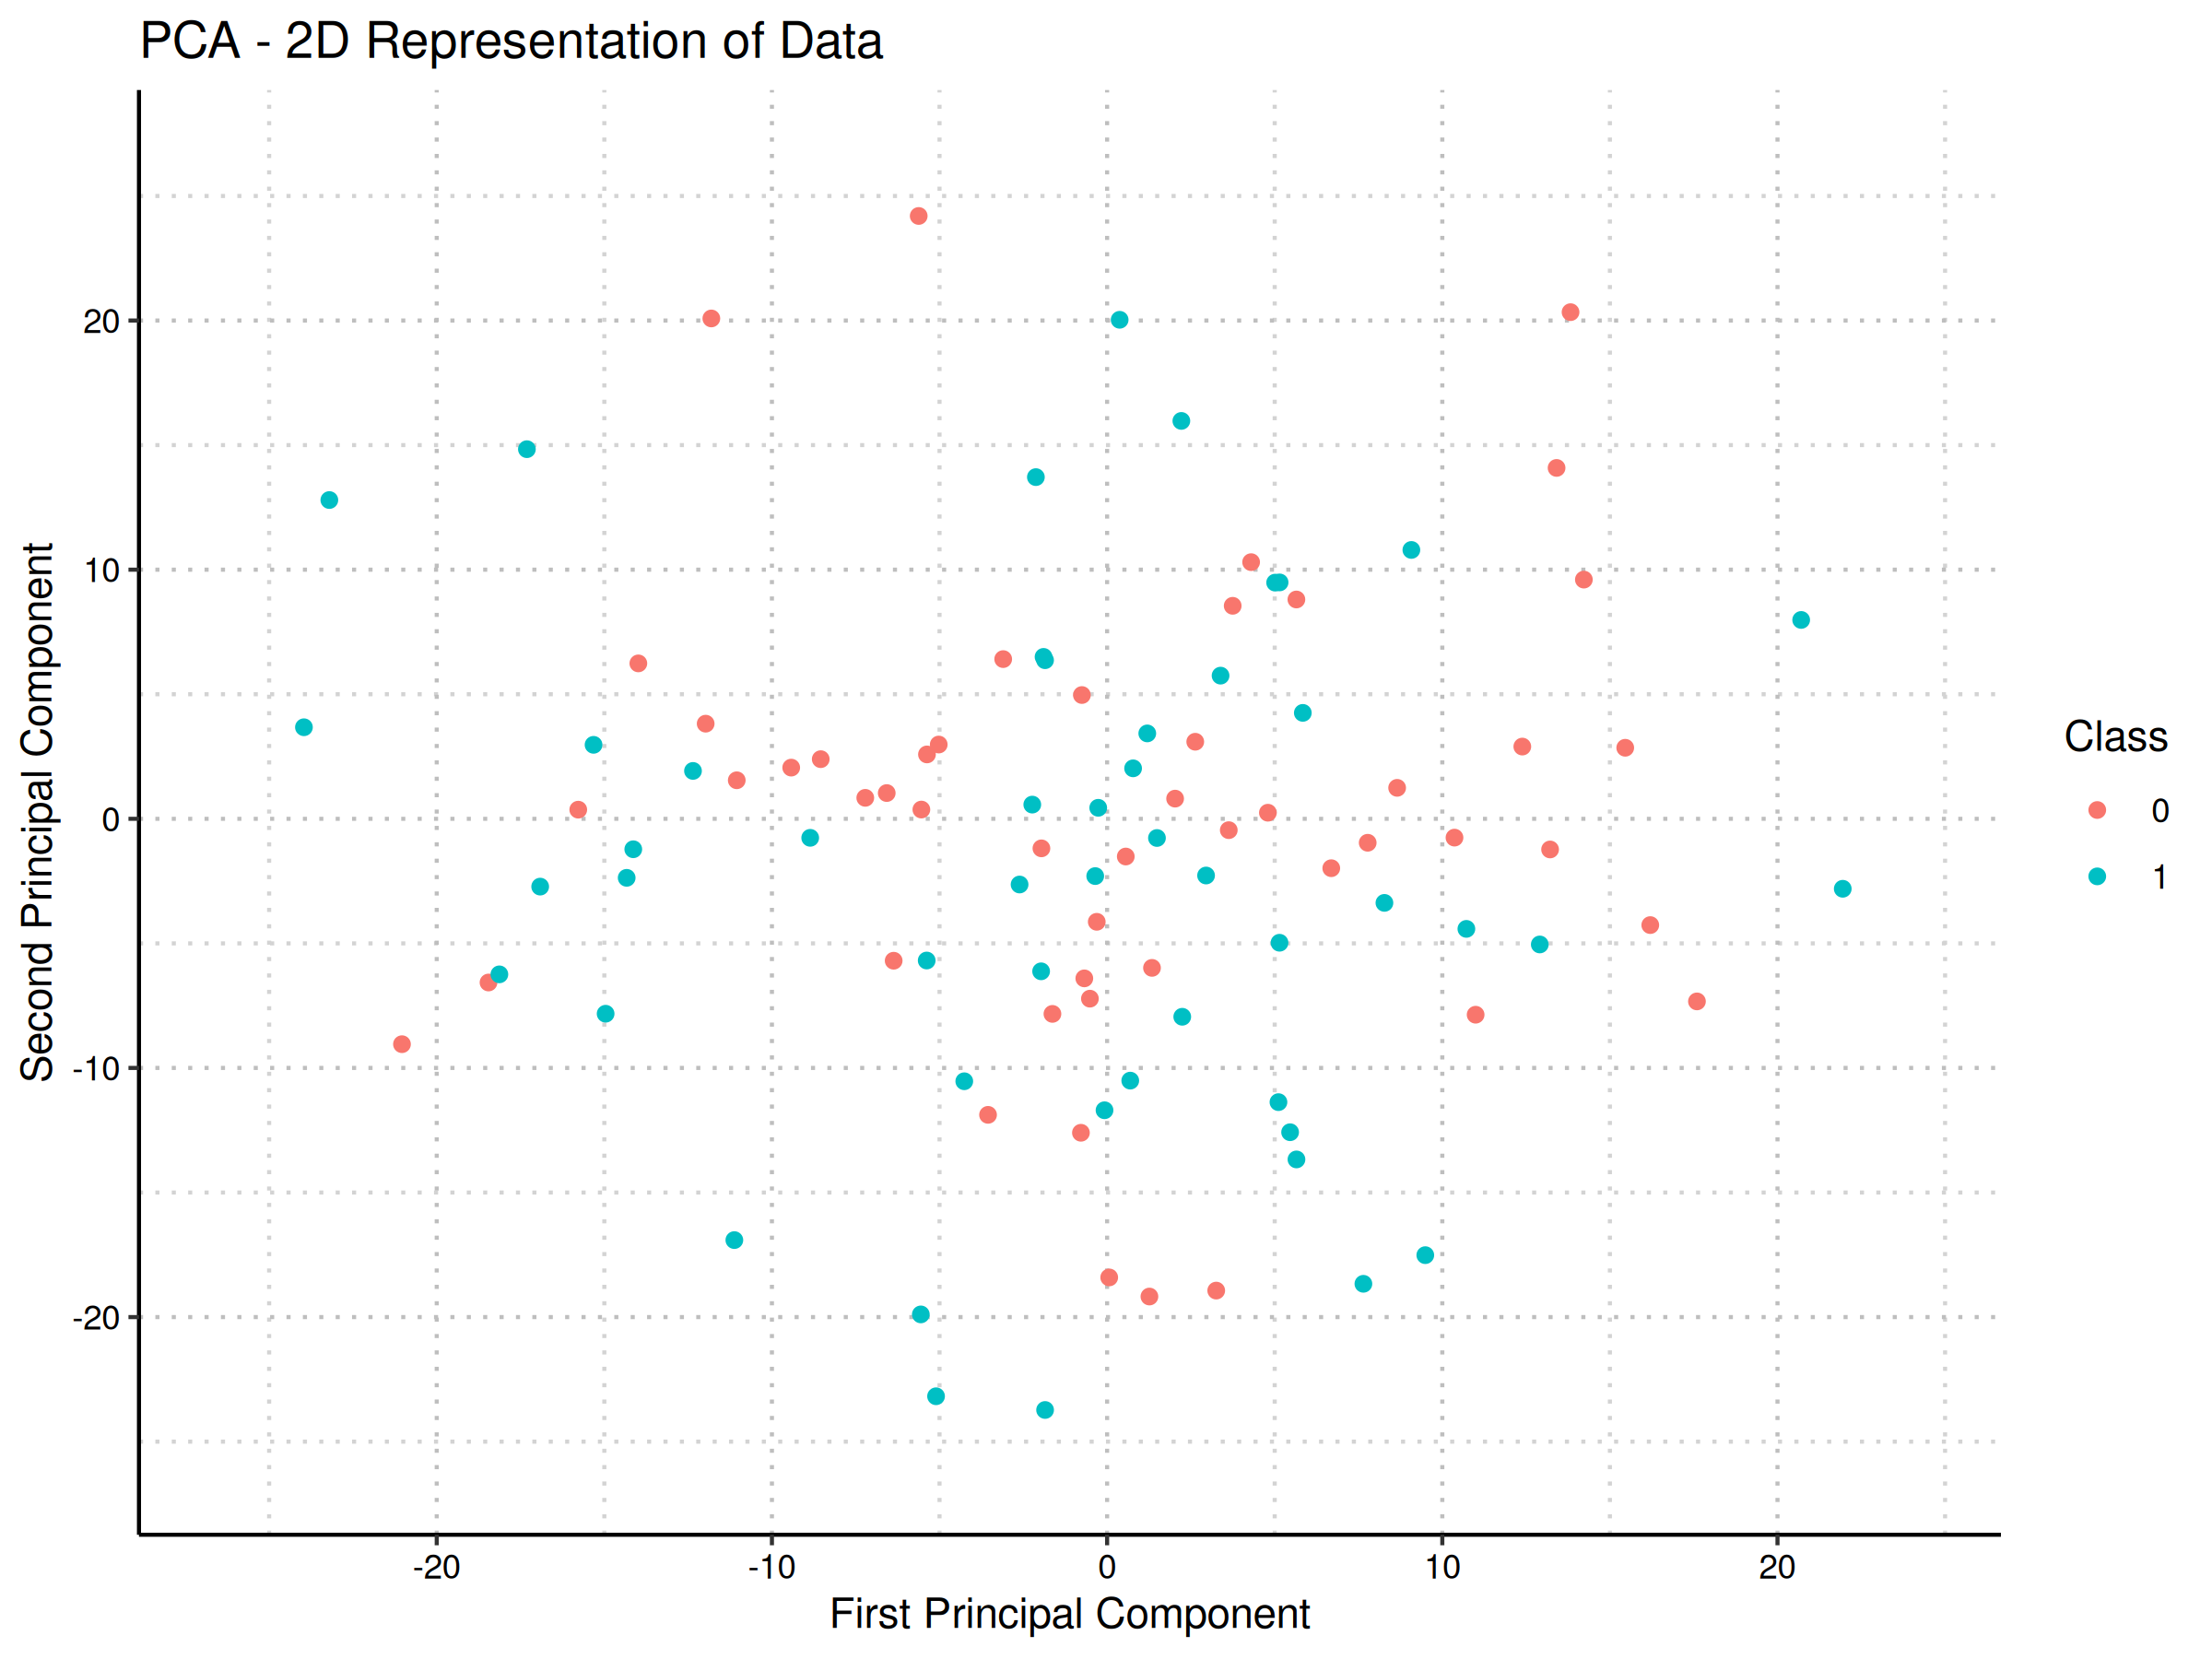
\includegraphics[scale = 0.5]{./images/clusters.png}
    \caption{Plane projection of the first two principal components of the explanatory variables simulated for 100 individuals when $\bm{\beta}^*$ is given by the concatenation of pictograms in Fig: \ref{fig:picto_blocs}
    \label{fig:compos_plan}}
\end{figure}



\newpage

\section{Real dataset}
\label{sec:real_data}

\subsection{Presentation of real data}

\noindent The actual data on which we are working comes from a cohort of 145 patients with liver tumors. 86 of them have HCC tumors, 22 have CCK tumors and 37 have mixed tumors. These proportions reflect the actual proportions of the different tumor classes in liver cancer patients. Each patient underwent four MRI radiographs of the liver, one at each time point after contrast injection. These were arterial, portal, venous and late. However, not all MRIs are usable. The patient may move during the MRI, rendering it unusable. A summary table (Table \ref{tab:nb_tumeurs}) is provided in order to specify the number of usable MRIs by temporality.\\
\indent Clinical data are also available: age at tumor detection, gender and patient alpha fetoprotein (AFP) levels. However, since the AFP levels of $22\%$ patients are missing from the data, we decided to exclude this clinical variable. As the gender of some patients (one with a HCC tumor, the other with a CCK tumor) was unknown, they were previously excluded from the study. The figures presented here and in the summary table Table \ref{tab:nb_tumeurs} show only those patients for whom we know the age at which the tumor was diagnosed and the gender.\\
\begin{table}[tbp]
    \centering
    \caption{Number of patients with usable MRI at the times indicated in the column for each tumor class. The total number of patients with each tumor class is entered in the total column.}
    \label{tab:nb_tumeurs}
    \begin{tabular}{|c|c|c|c|c|c|c|c|c|c|c|}
        \cline{1-7} \cline{9-9}
        class & Arterial & Portal & Venous & Late & All times & all times except venous& & total \\
        \cline{1-7} \cline{9-9}
        HCC & 84 & 81 & 83 & 78 & 72 & 74 & & 86\\
        \cline{1-7} \cline{9-9}
        CCK & 18 & 18 & 14 & 18 & 12 & 16 & & 19\\
        \cline{1-7} \cline{9-9}
        Mixtes & 35 & 36 & 32 & 34 & 29 & 31 & & 37\\
        \cline{1-7} \cline{9-9}
    \end{tabular}
\end{table}
\indent On each of the MRI, the tumor area is displayed and saved as a mask superimposed on the MRI. The MRIs and masks are in .nii format. Although taken at four different times, the four MRIs are very similar. In particular, the MRIs at venous and late time are extremely similar and often redundant in the eyes of radiologists. We will take this opportunity to eliminate the venous time MRIs, as this is the time for which there are the most missing MRIs.
We propose two possible extractions for features. A 3D extraction, where features are extracted from the entire tumor volume, and a 2D extraction, where features are extracted from each tumor section. These extractions are the result of a calibration in which we used the performance of a lasso-penalized logistic model as a reference (to know which features to add or remove).\\
\indent As previously mentioned, we will only study the distinction between HCC and CCK tumors, which allows us to directly use the binary classification models described in the “Machine learning models” section.(\ref{sec:models}). 

\subsection{feature extraction in 3D}
\label{sec:3D}

\noindent We use the pyradiomics package \cite{pyradio} to extract an array of 3D features for each tumor. Only the original (unfiltered) image is used to extract these features. We extract all the first-order parameters (relative to gray levels), 3D shape parameters (volume, surface, etc.), and texture parameters (based on co-occurrence matrix, gradient matrix, etc.) proposed by the package (except those considered deprecated or duplicative: for example, we eliminate glcm joint average as it is redundant with glcm sum average). The result is $106$ features for each radio. Shape parameters are averaged over all extracted temporalities, as we consider that the shape of a tumor has no reason to change between different MRIs.\\
\indent The exact parameters used for pyradiomics extraction are given in appendix \ref{annexeparam}. To ensure that the extraction is consistent from one tumor to the next, all tumors have been resampled to the same scale. On each $(x,y,z)$ axis, the spacing used is half the median spacing on that axis (calculated over all available MRIs). The idea behind this spacing is to avoid losing too much information by increasing the voxel size of higher-resolution MRIs without having to completely interpolate lower-resolution MRIs. Image interpolations are performed using cubic splines, while mask interpolations are based on the closest interpolation method (to guarantee mask connectivity).\\
\indent The advantage of 3D extraction is that each MRI image is summarized in a relatively small number of features (compared with 2D extraction). What's more, since the parameters are calculated on the tumor in its entirety, they do not omit any part of it. This idea is confirmed by the lack of improvement in the performance of the logistic lasso regression when features from the 2D extraction are added to the 3D parameters: the 3D features seem to stand on their own. The weakness of the 3D extraction is that it requires a complete segmentation by the radiologist of every tumor in the training database, which is very time-consuming.

\subsection{Feature extraction in 2D}
\label{sec:2D}
\noindent The first step in this extraction process is to determine the slices we wish to extract from the tumor. We choose the axial plane for the slices, as this is the one used by radiologists when analyzing a tumor. As for the extraction parameters, they are again given in Appendix \ref{annexeparam}. However, we cannot simply extract slices at regular intervals along the vertical axis, for two reasons:\\
\indent Firstly, tumor size varies from patient to patient. Thus, a certain spacing between slices will lead to the extraction of 3 slices of tumors in some patients and 10 slices in others. However, the machine learning models we use need to compare the same features in all patients. Secondly, slices with a very small piece of tumor are not very significant for our analysis. However, extracting at regular intervals will lead to the extraction of such slices at the beginning and end of certain elongated tumors (along vertical axis). We'd therefore like to give more importance to slices where the tumor is most present (without completely ignoring slices with less tumor on them).\\
\indent We therefore propose an extraction where we first specify the number of slices $n_{\text{slices}}$ to be extracted from each tumor. We begin by interpolating the cumulative distribution of tumor volume by depth (along the vertical axis) for each tumor (see Fig. \ref{fig:depth_volume}). This curve is then inverted to obtain the depth distribution as a function of the cumulative tumor volume covered. A slice is then extracted at each of the following depths: 
\begin{equation}
(i-0.5) \displaystyle{\frac{\text{area}_{\text{max}}}{n_{\text{slices}}}} \hspace{1.5 cm} \text{for i } \in \llbracket 1,n_{\text{slices}}  \rrbracket
\end{equation}
We have experimented other extraction methods, in particular trying to extract precisely the same depths for each MRI of the same tumor, while taking into account the fact that the patient may have moved slightly between two MRIs. However, as the results were of lesser quality, we will not develop these approaches here.\\
\indent The feature extraction used for each slice is almost the same as the one used for the 3D tumor (in the previous section), except for shape parameters. In fact, 2D shape parameters (instead of 3D shape parameters) are now extracted by pyradiomics. 2D shape parameters are always averaged over all MRIs of the same tumor (variations in tumor shape between MRIs result solely from changes in the way radiologists cut masks, and therefore do not provide information on the tumor itself).\\
\indent The advantage of this type of extraction is that the radiologist may only needs to segment a limited number of slices that are “representative” of the tumour, instead of the whole tumor. Indeed, the work carried out to find the right slices to extract could be replaced by an estimate made by the radiologist's naked eye. Although it would be necessary to check that the results are not affected by this change, this method seems simpler to generalize to large datasets (the segmentation of a couple of slices being less time consuming for a radiologist than the segmentation of the whole tumor). The disadvantage of this extraction method is that it loses the information contained in the slices that were not selected, as well as that concerning the overall shape of the tumor (which cannot be reduced to the shape observed on a few slices). This results in a slightly poorer performance of all models on these data \ref{sec:results}.

\begin{figure}[tbp]
    \centering
    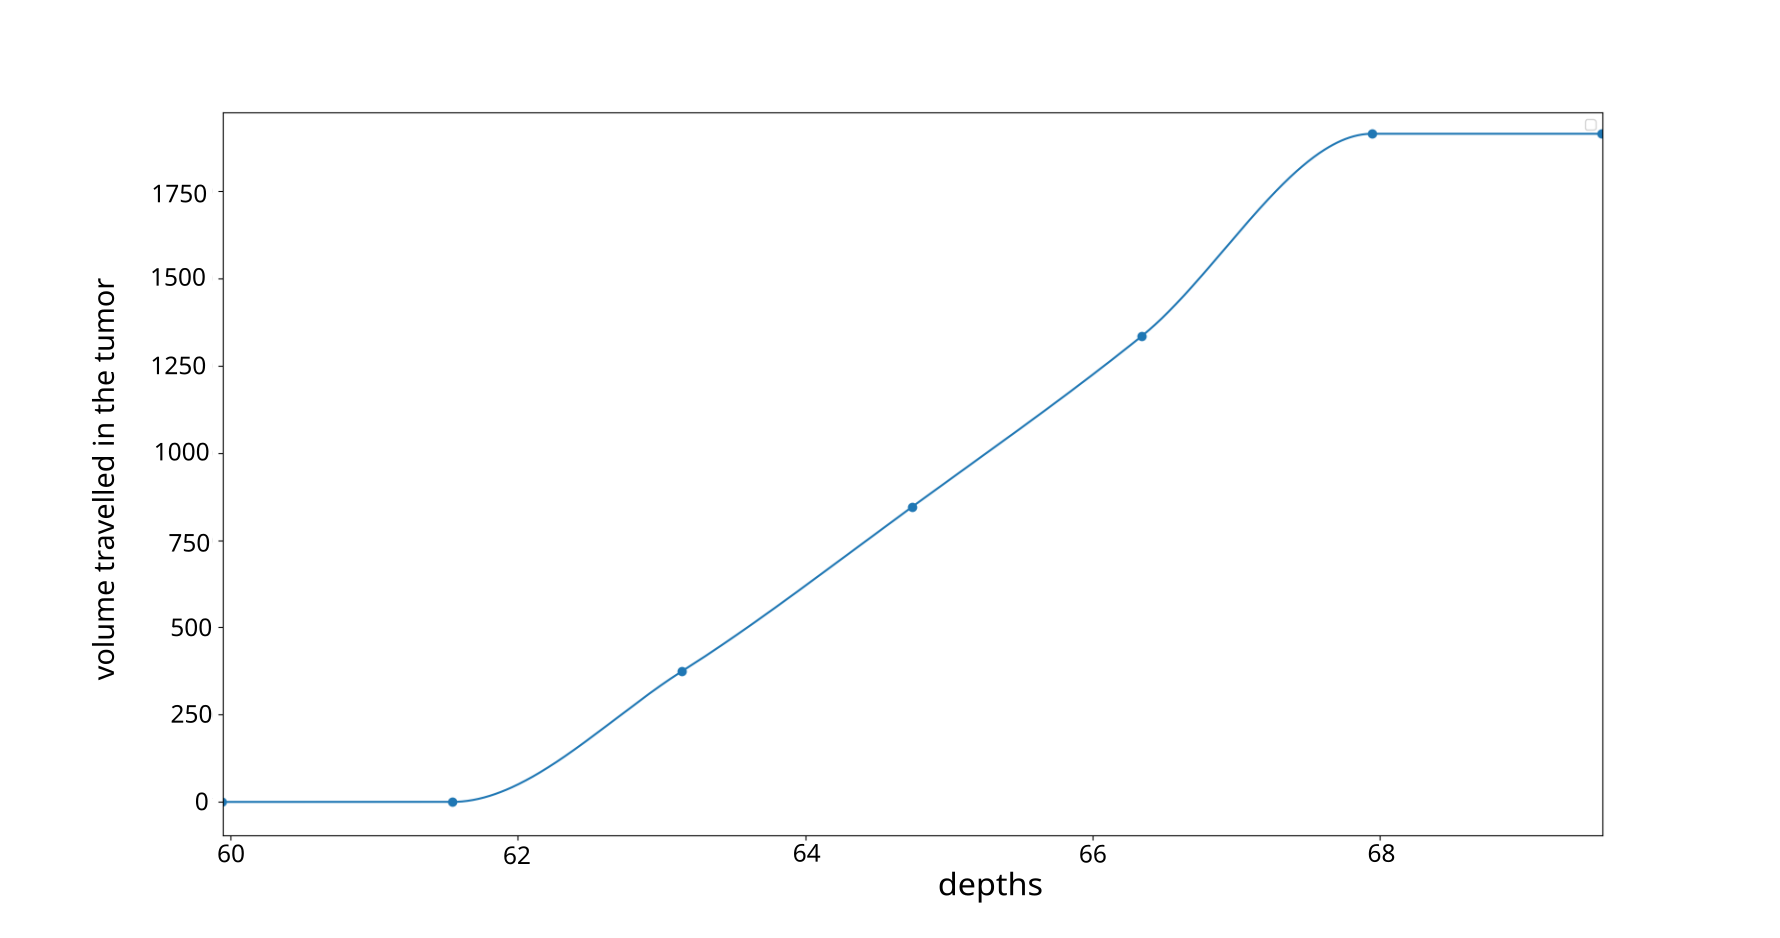
\includegraphics[scale = 0.25]{./images/plot_depth_volume_2.png}
    \caption{graph of the cumulative volume distribution (in $mm^3$) of the third CCK patient's tumor according to depth (in $mm$) for a given tumor. The points correspond to the slices recorded in the sitk image (with its initial spacing). The curve is obtained by interpolating these points using Hermite cubic splines.}
    \label{fig:depth_volume}
\end{figure}

\subsection{Extraction of healthy liver parts}
\noindent We wanted to add the features obtained by performing the extraction on portions of healthy liver. Radiologists generally compare the luminosity of the tumor area with the rest of the liver, so it seemed appropriate to do the same with our model.\\
\indent To do this, a small strip of tissue was extracted around the tumor area. To ensure that no area outside the liver or crossed by a blood vessel was included, we decided to extract only areas of low local variance and whose luminosity was greater than that of the black background. By adding a 3D connectivity criterion, we can extract a 3D area of healthy liver large enough to perform a 3D extraction of firstorder and texture features (the shape of the extracted area being of no interest).\\
\indent To ensure that the same area of healthy tissue was extracted from each MRI of the same tumor, we decided to crop the healthy tissue on the late MRI only (this was when our extraction method was most visually successful). We then applied the same trimming to the other MRIs, shifting the extracted area slightly to take account of the patient's movements. These movements were estimated by comparing the tumor areas on each slice and trying to increase as much as possible the intercorrelation of the area curves between each MRI and the late MRI. This procedure is performed along all three spatial axes. Finally, the extracted zone can be visualized, as in Fig. \ref{fig:healthy_zone} to check that the extraction is proceeding correctly.\\
\indent However, we did not perceive any improvement in the performance of our models by adding these features. We therefore decided not to include them in the rest of our study.\\

\begin{figure}[tbp]
    \centering
    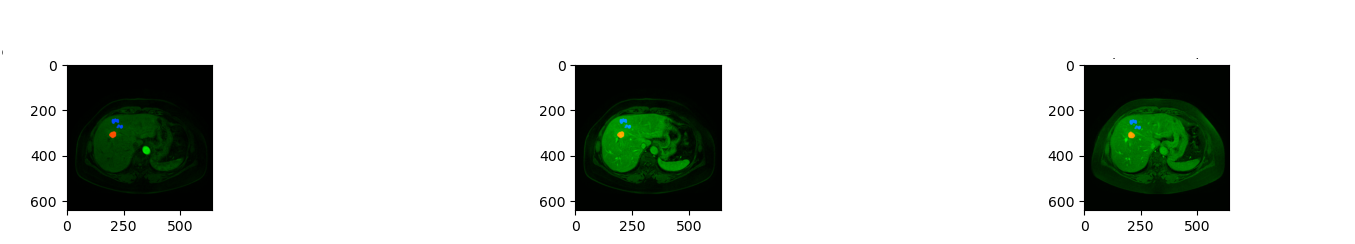
\includegraphics[scale = 0.5]{./images/sain.png}
    \caption{MRIs of a CCK tumor slice with the tumor area in red and the peripheral area of extracted healthy liver in blue. From left to right, arterial, portal and late MRIs. Axes are graduated in mm.}
    \label{fig:healthy_zone}
\end{figure}

\newpage
\section{results}
\label{sec:results}
\noindent In this section, we compare the performance of the tensor models presented in \ref{sec:models} with non-tensorial approaches, namely lasso and group lasso logistic regressions. These alternative methods operate directly on the unfolded matrix $\mathbf{X}_{(1)}$. To approximate the structure-awareness of tensor models, the group lasso is applied with feature grouping based on modes or variable names. This comparison allows to evaluate the potential performance benefits of explicitly preserving the tensor structure in the model.
\subsection{Simulated data}

\begin{table}[tbp]
    \centering
    \caption{Area under curve for each model on simulated data. For the group lasso model, it is possible to group variables by block, mode or variable. The type of grouping used is indicated in brackets}
    \label{tab:result_simul}
    \renewcommand{\arraystretch}{1.2} 
    \begin{adjustbox}{center}
    \begin{tabular}{|>{\centering\arraybackslash}m{2cm}|>{\centering\arraybackslash}m{2.5cm}|>{\centering\arraybackslash}m{2.5cm}|>{\centering\arraybackslash}m{2.5cm}|>{\centering\arraybackslash}m{2.5cm}|>{\centering\arraybackslash}m{2cm}|>{\centering\arraybackslash}m{2.5cm}|}
        \cline{1-7}
        number of individuals & lasso & goup lasso (by block) & goup lasso (by mode)& group lasso (by variable) & multiway & multiway multibloc\\
        \cline{1-7} 
        3000 & 0.83 & 0.86 & 0.94 & 0.94 & 0.99 & 0.99 \\
        \cline{1-7}
        500 & 0.59 & 0.65 & 0.64 & 0.63 & 0.92 & 0.63 \\
        \cline{1-7}
    \end{tabular}
\end{adjustbox}
\end{table}

\noindent We performed tests on simulated data generated with the parameters presented in \ref{annexe:hyperparam}. The pictogram to retrieve is the one in figure \ref{fig:picto_blocs}. We evaluated the performance in two settings: one with a lot of individuals to classify ($3000$ individuals in the training data set) and another with fewer individuals to classify ($500$ individuals in the training dataset). The testing dataset is always composed of $1000$ individuals. We consider the area under curve to determine the performance of each model as it is a robust and fine grained indicator of the efficience of each model to separate the two classes. We show the results in Table \ref{tab:result_simul}. For each model, the hyperparameters used during cross-validation are provided in \ref{annexe:hyperparam}. In each case, we present the pictogram reconstructed in \ref{annexe:picto}\\
\indent We can see that, in the presence of a large number of individuals (3,000), the multiway multiblock model is the most successful at reconstructing pictograms. In terms of performance, measured by the area under curve, its performance in this setting is similar to that of the multiway model. The other models (group lasso and classical logistic regression with lasso) perform much less well than the two tensor models.
In the presence of a small number of individuals (500), the multiway model performed best. In fact, it captures the pictogram structure in a very small number of parameters (the rank chosen by cross validation is equal to 1 in this configuration). Even imposing a rank of 1 on the multiway multiblock model requires the calculation of more coefficients (around $2$ times more in the case of our pictograms), which can lead to greater over-interpretation.\\
\indent These simulations clearly demonstrate the usefulness of tensor models for classifying high-dimensional data. They show that the structure of the $\beta$ coefficient is more easily found by the multiway multiblock model (when $\beta$ has a block structure, as is the case for our pictograms). However, results also indicate that the multiway model performs better than the multiway multiblock model in classification tasks when working with small datasets.\\

\subsection{real data}
\noindent We carried out tests on simulated data both using the 3D extraction (as described in \ref{sec:3D}) and the 2D extraction (as described in \ref{sec:2D}). Results are presented for each model in table \ref{tab:result_real}. All results are averaged over $50$ different training sessions. An analysis of the importance of each feature of the data studied is also proposed in \ref{annexe:importance}\\
\begin{table}[tbp]
    \centering
    \caption{Average area under curve obtained with each model on real data for 50 different trainings (with different partition between training set and testing set). For the group lasso model, it is possible to group variables by block, mode or variable. The type of grouping used is indicated in brackets. The confidence intervals provided are normal-based at a $95\%$ confidence level.}
    \label{tab:result_real}
    \renewcommand{\arraystretch}{1.2} 
    \begin{adjustbox}{center}
    \begin{tabular}{|>{\centering\arraybackslash}m{2cm}|>{\centering\arraybackslash}m{2.5cm}|>{\centering\arraybackslash}m{2.5cm}|>{\centering\arraybackslash}m{2.5cm}|>{\centering\arraybackslash}m{2.5cm}|>{\centering\arraybackslash}m{2cm}|>{\centering\arraybackslash}m{2.5cm}|}
        \cline{1-7}
        Type of data & lasso & goup lasso (by block) & goup lasso (by time)& group lasso (by variable) & multiway & multiway multibloc\\
        \cline{1-7} 
        3D & $0.74 \pm 0.04$& $0.78 \pm 0.03$ & $0.76 \pm 0.03$ & $0.73 \pm 0.03$ & $0.77 \pm 0.03$ & $0.77 \pm 0.03$ \\
        \cline{1-7}

    \end{tabular}
    
\end{adjustbox}
\parbox{0.9\textwidth}{
\vspace{0.2 cm}    
\centering \small Area under curve (AUC) on 3D real data}
\vspace{0.3 cm}

\begin{adjustbox}{center}
\begin{tabular}{|>{\centering\arraybackslash}m{2cm}|>{\centering\arraybackslash}m{2cm}|>{\centering\arraybackslash}m{2cm}|>{\centering\arraybackslash}m{2cm}|>{\centering\arraybackslash}m{2.5cm}|>{\centering\arraybackslash}m{2.5cm}|>{\centering\arraybackslash}m{2cm}|>{\centering\arraybackslash}m{2cm}|}
    \cline{1-8}
    Type of data & lasso & goup lasso (by block) & goup lasso (by slice)& group lasso (by time)& group lasso (by variable) & multiway & multiway multibloc\\
    \cline{1-8} 
    2D & $0.73 \pm 0.03$ & $0.71 \pm 0.03$ & $0.70 \pm 0.04$ & $0.71 \pm 0.03 $  & $0.71 \pm 0.03$ & $0.66 \pm 0.04$ & $0.71 \pm 0.03$ \\
    \cline{1-8}
\end{tabular}
\end{adjustbox}
\parbox{0.9\textwidth}{
\vspace{0.2 cm}    
\centering \small Area under curve (AUC) on 2D real data}
\end{table}
The performance obtained on medical data are not good enough for our models to be used in real conditions. In particular, in the course of our tests, we found that no model achieved an accuracy of better than $50\%$ in the detection of HCC tumors. Overall, 3D data give better results than 2D data. This may be explained by the fact that 2D data do not take into account the entire tumor. Experiments combining 2D and 3D parameters have been carried out, but have never exceeded the performance of 3D data alone.\\
\indent With both extraction procedures, the multiway multiblock model performs well compared to other models, but never better than all the studied non-tensorial models. This indicates that the structure of the optimal $\bm{\beta}$ parameter is likely not tensorial. Indeed, a simple grouping of features into groups (enabled by the group lasso), is sufficient to obtain similar results. In terms of computation time, the multiblock model is the most time-consuming, as it requires cross-validation on the rank to be used. In particular, as the number of times and slices in the data is close to $1$, there is no gain in computation time compared with non-tensor models.\\


\section{Conclusion}

The results obtained from simulated data show a clear advantage of tensor-based methods over non-tensor methods, attributable to the fact that the regression coefficient $\bm{\beta}_{\text{opt}}$ possesses a tensor structure. The multiway multiblock model is particularly well suited to finding the structure of the $\bm{\beta}_{\text{opt}}$ coefficient efficiently when the data are separated into blocks. But in any case, the classic multiway model offers the best classification performance. However, on the liver cancer data, tensor methods offer no particular advantage over other models. We can therefore assume that, while the features are well structured in tensor form, this is not the case for the $\bm{\beta}_\text{opt}$ coefficient. What's more, the results obtained on these data are far too weak to be exploitable in a medical context. These poor results can be explained by the lack of training data: there are only $16$ CCK tumors whose MRI images contain all the times studied.\\
\indent However, our approach to the real data studied has another limitation. We rely exclusively on pyradiomics to extract features of interest from MRI images of tumors. However, these features (gray levels, co-occurrence matrix, etc.) are more a matter of image processing than of medicine. Thus, they do not necessarily correspond to what radiologists would look at to classify liver tumors. It would therefore be interesting to train machine learning models on indicators constructed by radiologists and compare their performance with that obtained in this article. 

\newpage

\section{Latest results: not mentioned in the article}

\noindent As indicated in the summary of this internship report, two weeks ago I went to visit Sébastien Mulé at Henri Mondor Hospital to talk to him about the pre-processing of liver cancer data. It was then that he remembered the existence of another database concerning the liver cancers of the patients studied in the article. In fact, for each individual, the radiologist had also indicated the presence or absence on the MRI images of $13$ markers (presence of necrosis, presence of luminal enhancement in the late phase, etc.) which are usually used by radiologists to determine the class (HCC or CCK) of the tumor. This translates into $13$ binary variables in the database, to which we add the patient's gender. Unlike the features extracted by pyradiomics, the features in this database are based exclusively on medical criteria. Furthermore, each marker indicated by the radiologist takes into account all $4$ MRI images, whereas features extracted by pyradiomics only took into account one image at a time and were therefore extracted image by image. This explains why, unlike the features extracted by pyradiomics, those in the new database are not tensorial.\\
\indent In order to compare these data with those studied in the article, a lasso logistic regression was performed on these data. Averaging the area under curve over $50$ trainings, we find:
$$
\text{AUC} = 0.96 \pm 0.02 \hspace{60 pt} \text{balanced accuracy} = 0.85 \pm 0.05
$$
where confidence intervals are of the normal type and calculated at the $95 \%$ threshold. We can see that the two most important features in the classification (where feature importances are calculated as in \ref{annexe:importance}) are, in descending order, late luminal enhancement and non-peripheral washout. The first of these two features is considered the most important by radiologists, which is consistent with our model. These results are much better than those obtained with data extracted by pyradiomics. The quality of these results is particularly high given the low number of patients in the training database. Moreover, lasso logistic regression may not be the best model on these data, and we can hope to improve these results still further by using models more suited to binary data (such as random forest). These results are left out of the article section for the following reasons:
\begin{itemize}[label = $\bullet$]
    \item They have no connection with tensors, whereas tensors are at the heart of the article. In order to practice writing reports in article format, it was therefore decided that I should write the section on actual data as if the latest data had not been communicated to me.
    \item As these results were obtained late in the course, we did not have much time to develop them. They cannot therefore be presented in the article.
\end{itemize}
I am well aware, however, that the latest results completely exceed those obtained in the article, and that, with a view to publication, it would be necessary to study another set of real data, more suited to tensor models.

\section{Retrospective and Perspectives on the Internship}

\subsection{Possible extensions of the work}

The work carried out on tensor models during this course shows that these models can be genuinely useful when the regression parameter has a tensor structure, as in the simulated data. However, the multiblock approach chosen in this internship may finally not be the most promising. Indeed, the primary objective of classification models is often to achieve optimal performance, rather than precisely reconstructing the structure of the regression parameters. In this area, the multiway model already developped in \cite{multi_rank_r} offers a real advantage over the multiway mulktiblock model presented in this report. But other approaches remain unexplored. We could change the penalty used to, for example, mix the L1 and L2 penalties, or mix the group lasso with tensor models. We could also try to adapt variable selection procedures such as those proposed in \cite{sis}, to improve computation speed in very high-dimensional tensors.\\
\indent With regard to the liver cancer data, it would be interesting to train several tabular machine learning models on the latest data (random forest, group lasso, boosting etc...) in order to propose the most accurate model possible and compare it with the methods already used by radiologists. Indeed, while the performance of the algorithms on the data presented in the article section of this report left no doubt as to their inferiority to that of radiologists, on the new data, this becomes more uncertain. Finally, it would also be good to add mixed tumors to the analysis, to see whether the models are also capable of distinguishing them. In practice, they make up around a fifth of tumours, and even if they are less well understood than HCC or CCK tumours, it remains interesting to be able to distinguish them.\\

\subsection{Assessment and Reflection}

\noindent This internship enabled me to acquire the technical skills needed to pursue a thesis under the right conditions in the same laboratory. Indeed, I was able to familiarize myself with complex classical machine learning models, with the R language, with tensor data and with the laboratory's calculator (and its formalism). As the data I will be working on in my thesis (the results of blood samples analysis taken from lung cancer patients) are of a similar nature to those studied in this internship (even if they will be of better quality), I will be able to reuse most of these tools. What's more, I have been able to see how the laboratory is organized and I am used to working with my supervisors. In particular, I think I have found the right balance between taking the initiative and asking my supervisors for help.\\
\indent I was also able to see how the distance between the various players could complicate the process of obtaining results. Indeed, I did not wait for the appointment at the hospital a few weeks before the end of the internship to meet Sébastien Mulé. On the contrary, he came to the laboratory regularly (around once every six weeks) to discuss research progress. But at no time did we think to ask him if data other than that which he had provided were available. And it was only at the hospital that he thought to mention the existence of such data. I think there are several reasons for this situation:
\begin{itemize}[label = $\bullet$]
    \item On the one hand, our distance from the hospital meant that our work was necessarily compartmentalized from that of the radiologists. This compartmentalization was accentuated by the fact that we had only one medical intermediary: Sébastien Mulé. As a result, the slightest omission on his part could have major consequences for our work (since we could not cross-reference our information with that of other radiologists).
    \item Furthermore, as my research placement was not part of a larger project, there was no dedicated project manager. My supervisors were the closest to this role, but they did not have the freedom to go out to the hospital regularly to talk to the doctors, as a project manager might have done. This had consequences for the flow of information.
\end{itemize}
\indent For my thesis, I will be keeping a close eye on these points, to make sure I do not miss out on any key information. So, with my supervisors, I will make sure I regularly meet as many stakeholders as possible (doctors, other PhD students working on the same data but from a different angle, their supervisors etc...), preferably at their place of work, to make sure I do not make any mistakes or forget anything. The question of the project manager should be less of an issue as the thesis I am about to pursue is part of a project with the Gustave Roussy foundation. As such, there is already a project manager in charge of coordinating the various research projects. My supervisors have already given me the opportunity to learn more about the project by inviting me to a progress meeting with all the stakeholders on Thursday September 26, 2024. \\
\indent Apart from the complexity of managing the risks associated with communicating information between the laboratory and the hospital, the management of other risks proved satisfactory. In fact, I regularly backed up my work on a GitHub server to ensure that I would not risk losing everything in the event of a problem with my personal computer. I also had an external hard disk on which I saved my work (albeit at less regular intervals), to avoid any major data loss in the event of a GitHub handling error. In addition, any demonstration written down on paper had to be quickly written up in LaTeX (a requirement of my supervisors), to avoid, for example any loss of time in the event of the research notebook being lost. As far as the risks associated with managing deadlines were concerned, we were also quite successful in planning the use of the calculator well in advance (more than three months before the end of the course). This turned out to be essential, because between the cyber-attack suffered by the University of Paris-Saclay, the calculator taking longer to get used to than expected (requiring lengthy discussions with the technical department) and maintenance lasting two weeks instead of one, I might never have had time to carry out my simulations if we had started later.\\
\indent The work carried out as part of this internship is useful for both the laboratory and the hospital. Trainings with simulated data on the multiway multiblock model are interesting, both for assessing the model's performance and for reflecting on data generation. For the hospital, the results obtained on the new real data set are promising, and encourage further research in this direction. Finally, although the work carried out on pyradiomics did not produce satisfactory results, it did enable us to exclude this extraction method from the scope of our studies. Indeed, the features obtained by pyradiomics had already been the subject of several research activities/projects with students at Centrale-Supélec or Henri Mondor hospital (master's thesis at Henri Mondor hospital, integration teaching at Centrale-Supélec etc.) and it was therefore important to discover their limits. This internship report condenses all the important information obtained during the internship, and will serve as a reference for the laboratory in the years to come, should any questions arise about the work that has been produced. In order to be as precise and concise as possible (and therefore as useful as possible for the laboratory), the research content has not been simplified in the article section.\\
\indent On a personal level, I am convinced of the merits of the research I have carried out. Machine learning is indeed the subject of much debate, and I would not have wanted to get involved in a project whose consequences could have been harmful to society. For example, the research I carried out was primarily aimed at improving a precise diagnosis, and not at replacing the radiologist (whose role goes far beyond this task). What's more, classic machine learning models such as those studied do not have the opacity of deep learning models, and remain highly specific. Nor do they have the invasive and potentially uncontrollable character of more “general” intelligence models such as language models. Finally, from the patient's point of view, it is important to note that the data used in this course are anonymized and that patients have given their consent for their RMI images to be used for research purposes.

\subsection{Competency framework}

\noindent In accordance with Centrale-Supélec's requirements for internship reports, this section presents a self-assessment of the engineer's nine skills, based on the experiences I had during this internship..\\

\subsubsection{Complexity}
\noindent \textbf{Statement}: \textit{ Analyze a system in its entirety, identify its scientific, economic, human and other dimensions, model with the appropriate scale and assumptions, solve the problem, and design all or part of a complex system.}\\[3 pt]

\noindent \textbf{Strengths}: I have worked with complex problems during this research internship and I have been able to adapt to studying them. In particular, I know that there is never just one solution to these problems. In the case of machine learning, sometimes it is the model that is at fault, other times the raw data, other times the pre-processing of this data, sometimes even the hardware used etc. So I have learned to be patient and not to close off possibilities from the outset. In particular, I think I have also grasped the human aspect of these problems, and the importance of good cooperation between all the parties involved in finding workable solutions.\\[3 pt] 

\noindent \textbf{Areas for improvement}: I have not often been confronted with problems with a strong economic component. Even if I integrate budget constraints into my projects (this will be the case, for example, for the lung cancer monitoring tool we will be developing during my thesis), I have never had to make decisions that would have major economic consequences. I still have a lot to learn in this respect. On the other hand, as I am at the very beginning of my professional career, I have to remain humble about my knowledge of complex problems: I believe that experience is also a key element in solving them.

\subsubsection{Engineering Profession}

\noindent \textbf{Statement}: \textit{In-depth knowledge of a particular discipline or sector should enable graduates to delve deeply into a field, to think in depth, to understand the difficulties and subtleties of a subject. This “expert” approach enables graduates to acquire complex ways of thinking that can then be transposed to other sectors, giving them the distance they need to approach future learning effectively. 2 axes are targeted: the business sector, and the cross-functional business line.}\\[3 pt]

\noindent \textbf{Strengths}: During this internship and my third year at Centrale-Supélec, I was able to deepen my knowledge of machine learning. In doing so, I was also able to make progress in mathematics, modeling and computer science, and I got into the habit of reading scientific articles on my own on subjects related to my work. I have also been able to discover the health sector and health research, which was previously unknown to me. All this gives me a more global vision, both of my field of expertise (I can deal with more machine learning problems, I know more about the “tricks”, the recurring difficulties etc.) but also of the field of engineering sciences in general (by being at the interface of several professions).\\[3 pt]

\noindent \textbf{Areas for improvement}: My versatility, linked to my engineering training, certainly enables me to adapt easily to a wide range of professional environments, but it has prevented me from delving as deeply into a specific field as students who have completed a full master's degree in it. For example, my specialization in machine learning only began in my final year at Centrale-Supélec, whereas other university students had studied the field for several years. I am particularly lacking in knowledge related to the mastery of low-level programming languages, web tools and concepts, containment, compilation and advanced use of Linux (although I am bound to make progress on these subjects as I continue in machine learning).

\subsubsection{Innovate and Undertake}

\noindent \textbf{Statement}: \textit{Entrepreneurial competence is understood in a broad sense (self-entrepreneur, capacity for action, intrapreneur, business creator, etc.): observing and allowing oneself to criticize the world as it is, questioning one's initial hypotheses, proposing alternatives integrating risks and uncertainty, concretely implementing innovative ideas, industrialization to deliver tangible results.}\\[3 pt]

\noindent \textbf{Strengths}: My research work (during this internship and during my research course at Centrale-Supélec) has accustomed me to proposing innovative solutions. In particular, I know that I should not hesitate to question the initial hypotheses of a given problem and to propose alternatives (as was the case for the processing of real data during this internship). I also know that before trying to innovate, you have to be sure of what already exists and try above all to reduce the difficulty of the problem posed (especially when you do not need an optimal solution). Finally, working with a hospital has taught me the importance of always keeping the customer's final objective in mind (to avoid any drift).\\[3 pt]

\noindent \textbf{Areas for improvement}: I have never been in an entrepreneurial or managerial context, so I have not often had to make decisions that impact an entire business. Nor have I had to manage teams of workers. So the human aspect of innovation contexts is still rather theoretical for me.

\subsubsection{Value Creation}

\noindent \textbf{Statement}: \textit{Starting from a company's definition of increased productivity and profitability, Value Creation is extended here to the contribution of progress and improvement in areas such as the efficiency of a process, the performance or reliability of a technical solution, or the environmental or societal impact; in such a way that the beneficiary (or beneficiaries), whether individual or collective (companies, organizations, society), can see and measure the effects.}\\[3 pt]

\noindent \textbf{Strengths}: I have already carried out group projects at Centrale-Supélec in response to a client's request (in the Major Project Management program, for example), and this internship was an opportunity to discover a scientific context where the major issue is added value for the client (the hospital). I know that it is important to clearly define the customer's expectations by discussing them with him beforehand. In particular, I have noticed that the customer is sometimes unaware of the extent of the possibilities available to him, and so it is important to be proactive during the exchange (this was the case here, for example, when we decided to study portions of the healthy zone in the tumor: Sébastien Mulé was not sure that we had the means to properly cut out these healthy zones ourselves). Defining evaluation metrics was also an important step at the start of the research internship, so I think I am pretty comfortable with this aspect.\\[3 pt]

\noindent \textbf{Areas for improvement}: I have never had to manage a major project, so I have not had to deal with the way in which these projects can gradually drift out of line with the customer's expectations. Furthermore, I have never had to deal with a situation where meeting the customer's expectations was linked to high financial stakes. I think I still need to gain experience in these areas.

\subsubsection{Intercultural}

\noindent \textbf{Statement}: \textit{ Evolve in multicultural and multilingual environments that expose you to ways of thinking, functioning and communicating that are different from your own, and step back from your own cultural filters to adapt, cognitively, behaviorally and emotionally, to intercultural environments.}\\[3 pt]

\noindent \textbf{Strengths}: This internship did not have any international component. In order to develop an answer on my current skills on this subject, I must call upon my international experience during the second semester of my gap year. It was an humanitarian internship in Greece, during which I had to adapt to the language barrier (I do not speak Greek) as well as to ways of thinking that were sometimes different from my own (although having remained in the European Union, apart from a generally more assertive conservatism than in France, I did not perceive any huge differences). During this internship, I was able to work with children of different nationalities and see how a humanitarian project was organized on several continents. Therefore I know what it means to work in a multicultural environment.\\
\indent I am fluent in English (level C1) and German (level B2) and I have already had the opportunity to work with people of different nationalities in a scientific context at Centrale-Supélec.\\[3 pt] 

\noindent \textbf{Areas for improvement}: I have never had to work in a country where the culture was completely different from my own (on another continent). What's more, my command of English, while good, is far from perfect, and I still have to rely heavily on automatic translators when I write a text.

\subsubsection{Digital}

\noindent \textbf{Statement}: \textit{Digital technologies are developing at breakneck speed, and their adoption by individuals and businesses is transforming the economy and society, introducing more sharing, cooperation and empowerment. This movement is accelerating and leading companies to transform themselves, or disappear. This transformation is not only technological, but also organizational and cultural. Students are at ease in this digital world where they innovate and “disrupt”. They understand the techniques and sciences that underpin the digital revolution.}\\[3 pt]

\noindent \textbf{Strengths}: Being specialized in machine learning, I am used to working with numerical methods, both for minimizing objective functions (as was the case during this internship) and for approximating densities. I also know that it is important to check their effectiveness in simple cases, by evaluating their margins of error and comparing them with existing methods wherever possible (as was the case when comparing the different regression models in this internship). Although it was not the focus of this internship, I know the basics of algorithm proofs and have taken specific courses on them in the context of optimization algorithms.\\
\indent I am also aware of the constraints linked to the performance of machines and calculators, and I have learned to make the best use of available capacities (by parallelizing calculations, for example) or by using common strategies (recall tables, approximations, etc.) to save calculation time. I am aware of the importance of not using more resources than necessary for calculations (this is expressly requested when using the laboratory's calculator, for both environmental and financial reasons). Finally, during the many group projects I carried out at Centrale-Supélec, I got into the habit of using collaborative work tools such as git (a tool also used during this internship) and of using the correct version for each tool (very important during this internship for pyradiomics to work: it does not function with the latest versions of Python).\\[3 pt]

\noindent \textbf{Areas for improvement} I never did software development or web development, and I have never taken a course on cybersecurity. I have already touched on these notions from afar during generic first and second year courses, but that's about it. However, I will probably end up having to learn more about these subjects if I want to continue in computer science. I have more knowledge of databases, but I have never needed to use or build one in SQL during my projects. Finally, I have never had to work with massive data, so I have not had to use big data tools like Hadoop or Spark (although I did take a course on them in my second year). Again, I think I will probably have to learn more about these subjects if I want to continue in machine learning.

\subsubsection{Persuade}

\noindent \textbf{Statement}: \textit{Convincing means presenting a point of view - or a proposal - in such a way as to enable an interlocutor to recognize its accuracy, relevance or force, and thus to appropriate it.}\\[3 pt]

\noindent \textbf{Strengths}: Writing this internship report (article section) gave me the opportunity to test myself against the requirements of a written scientific presentation. In particular, the methodology section, which was written before the rest of the report, underwent several revisions to make it more precise, which gave me a good idea of the level of clarity expected in a publication. During this internship, I also often had to present my latest advances to my supervisors orally, sometimes without any written support, and I think I have made a lot of progress in this area. I am now better at justifying my choices and anticipating objections. Finally, this internship has forced me to adapt to my interlocutor, for example by simplifying mathematical explanations when talking to a doctor.\\[3 pt]

\noindent \textbf{Areas for improvement}: I need to take more into account readability in my reports. Indeed, I have often tended to write equations that are too heavy with too few comments in the Methodology section, which can put off an uninitiated reader (this is what required the most corrections in the article part of this report).

\subsubsection{Project Team}

\noindent \textbf{Enoncé} \textit{Build, mobilize and train a collective to work as a team, demonstrate different forms of leadership, enrich the team with external resources and expertise, and work in project mode.}\\[3 pt]

\noindent \textbf{Strengths}: Since no other intern or PhD student was working on my research topic, the leadership and task distribution aspect was less present than in other internships. However, I quickly understood that it would be necessary for me to be proactive, by regularly making decisions myself and testing my proposals before submitting them to my supervisors. In addition, I also realized that I had to question my supervisors' proposals and not hesitate to ask them for details on the real expectations of each task. This was the case, for example, in the pre-processing part of the real data, where I was able to discover several points where the extraction of the real data was suboptimal (some parameters to be extracted were omitted, there were different scales for each RMI image of the same patient, etc.)\\[3 pt]

\noindent \textbf{Areas for improvement}: The communication with the radiologist could have been improved, which would have avoided us changing real data a few weeks before the end of the internship. In addition, even if my internship was not considered as a project, in the sense that the final goal was only to have the best possible results and not to develop a finished tool, an organization closer to project management could probably have helped. In particular, giving one of the two supervisors the full responsibility of project manager would have probably helped communication. However, I think that from a logistical point of view (the supervisors are already researchers themselves and also supervise doctoral students, the hospital is far from the laboratory, etc.), this was not possible.

\subsubsection{Ethics and Sustainability}

\noindent \textbf{Statement} \textit{Analyze and anticipate the possible consequences of one's actions, of the decisions of organizations and economic models of the structures to which one contributes; arbitrate an ethical dilemma; act in an inclusive manner when faced with questions of diversity; respect scientific ethics.}\\[3 pt]

\noindent Ethical questions cannot be reduced to binary reasoning (strengths/areas for improvement) so this separation is abandoned here.\\
\indent The main ethical dimension of this internship concerns the impact of the research carried out. Indeed, machine learning is a powerful tool whose use can be negative on our society. For example, we can think of the use of language models by foreign powers to write waves of negative comments under political articles or videos or the impact of the recommendation algorithms of Youtube, Facebook or Twitter, which tend to imprison users in filter bubbles (by only showing them what confirms their position) and amplify the sharing of hateful and misleading content compared to other content. In this internship, however, this type of use is not really possible. Indeed, most of the algorithms that are debated are based on deep learning (artificial neural networks), which is not the subject of this internship. Furthermore, the algorithms developed here are specific to a certain type of data and it therefore seems unlikely that their use will be diverted for malicious purposes. On the contrary, we can guess the immediate interest of the research carried out, namely the improvement of the diagnosis of liver cancer. In my opinion, therefore, the ethical impact of this internship is positive.\\
\indent Furthermore, since the data is anonymized and was collected from patients who gave their consent for their RMI images to be used for research purposes, this data is collected ethically. Furthermore, as stated earlier in this report, there is no question of replacing the work of a human being with this type of model. And even by extending this type of work, it seems difficult to imagine arriving at models capable of replacing humans (these models learn a specific task and are not capable of generalizing to other tasks). Finally, regarding this report itself, I was careful to write it as accurately as possible, without modifying or exaggerating the results obtained, even when it did not go in the direction I would have initially hoped.

\newpage

\section{Acknowledgments}

\vspace{2em}
I warmly thank my two supervisors Arthur Tenenhaus and Laurent Lebrusquet for their kindness and availability throughout this internship. I also thank them for the motivation they helped give me in this research work, even when the results were not those expected. I thank them for accepting after this internship to welcome me in this laboratory where I feel so good since the beginning of this internship. Finally, I thank them for all the help they gave me during this internship, whether on the computer, mathematical or administrative level.\\[1em]
\indent I thank Sébastien Mulé for the time he was willing to devote to us in addition to his working hours, despite his already very busy schedule, and for all the trips he agreed to make to the laboratory. I also thank him for the many explanations he gave us about liver cancer and for his offer to host me in his hospital for a day (which led to the discovery of the new database studied).\\[1em]
\indent Finally, I would like to thank the technical support of the laboratory calculator, without which the simulations could not have been carried out.

%% The Appendices part is started with the command \appendix;
%% appendix sections are then done as normal sections

%% For citations use: 
%%       \cite{<label>} ==> [1]

%%

%% If you have bib database file and want bibtex to generate the
%% bibitems, please use
%%
\newpage
 \bibliographystyle{elsarticle-num} 
 \bibliography{bibliography.bib}

%% else use the following coding to input the bibitems directly in the
%% TeX file.

%% Refer following link for more details about bibliography and citations.
%% https://en.wikibooks.org/wiki/LaTeX/BiblD iography_Management

\newpage

\appendix

\section{Hyperparameters for simulated data}
\label{annexe:hyperparam}
\subsection{Data generation}

\noindent In our simulations, we unfold the $\beta^l$ of each pictogram line by line into a vector (rather than a matrix) and concatenate these vectors to obtain $\bm{\beta} = [\bm{\beta}^1; \; \hdots \; \bm{\beta}^L]$. Let $N$ be the size of $\bm{\beta}$. We then use the following parameters to generate the simulated data:
\begin{itemize}[label = $\bullet$]
    \item $\bm{\mu}_0 = \mathbb{0}_N$
    \item $\bm{\mu}_1 = \bm{\beta}/\lVert \bm{\beta}\rVert$ 
    \item $\mathbf{P}$ is obtained by completing in orthonormal basis $\bm{\beta}/\lVert \bm{\beta}\rVert$
    \item $d_1 = 0.01$
    \item For $i \in \llbracket 2, N \rrbracket$, $d_i = 0.25$ (where ($d_i$) are the diagonal elements of $\mathbf{D}$) 
\end{itemize}

On $1000$ individuals generated, with 500 in each class, the accuracy obtained by the 2-means algorithm is $0.48$: in other words, it doesn't do better than chance (even slightly worse in our case). However, the section \ref{sec:results} shows far better performance from our models

\subsection{Cross validation of models}

\noindent For the lasso and group lasso models, we cross-validate on $20$ values of $\lambda$ distributed according to a logarithmic scale between $10^{-5}$ and $10^{-13}$.\\
\indent For the muliway and multiway mulibloc models, we cross-validate on $5$ values of $\lambda$ distributed on a logarithmic scale between $10^{-3}$ and $10^{-6}$. We also cross-validate on the rank used. The rank of $\bm{\beta}^*$ is bounded above by the sum of the ranks of the individual pictograms (around $15$, $1$ and $10$ respectively). So we won't exceed $27$ for rank in our cross validation. In fact, we hope to approximate $\beta$ with a matrix of rank lower than $26$ to ensure a certain sparsity in the model. We therefore cross-validate on ranks $1$, $10$ and $20$ in the multiway model (to propose a model parameterization with a minimal rank, an intermediate rank and a high rank).\\
\indent In the multiblock model, you can choose a rank for each pictogram. In order not to overload the cross-validation, we limit ourselves to cross-validating on the rank of the first pictogram. As this is the highest-ranking pictogram, there are more different “choices” possible for the multiblock model, depending on the desired sparsity. We therefore propose the ranks $1$, $6$ and $12$ for this pictogram in the cross validation. For the other pictograms, we impose $1$ and $10$ respectively. Here again, we also cross-validate on $5$ values of $\lambda$, distributed on a logarithmic scale between $10^{-3}$ and $10^{-6}$.





\newpage

\section{Parameters used for feature extraction with pyradiomics}
\label{annexeparam}

List of parameters used for feature extraction by pyradiomics:
 
\begin{itemize}[label = $\bullet$]
    \item Bin width : 25
    \item Resampled Pixel Spacing : $[2,2,2]$ si l'extraction est en 3D, $[2,2]$ si elle est en 2D
    \item interpolator : sitkBSpline
    \item force2D : True
    \item force2Ddimension : 2
\end{itemize}


\section{Reconstructed pictograms}
\label{annexe:picto}

\begin{figure}[H]
    \centering
    \begin{tabular}{cc}
        \subfloat[lasso \label{fig:3000simple}]{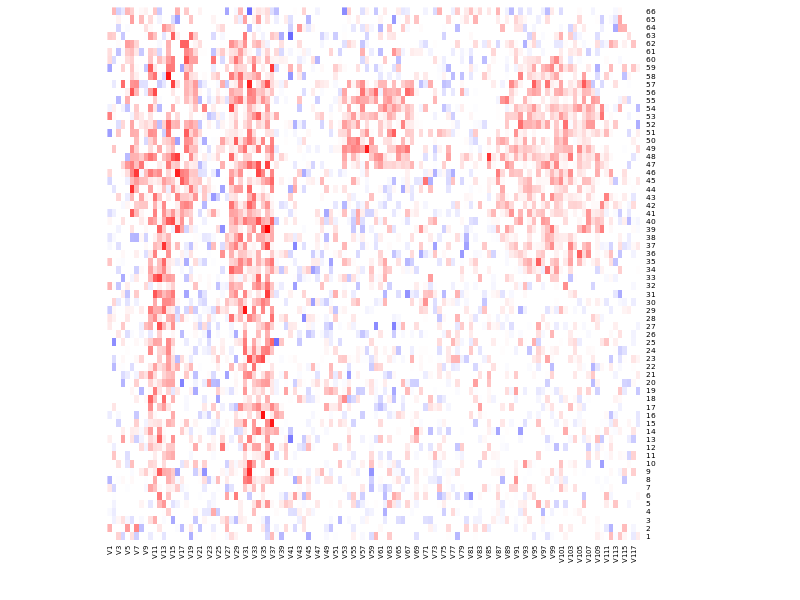
\includegraphics[width=0.35\textwidth]{images/heatmap_logistique_simple_simu_4000.png}} &
        \subfloat[group lasso (block)\label{fig:3000bloc}]{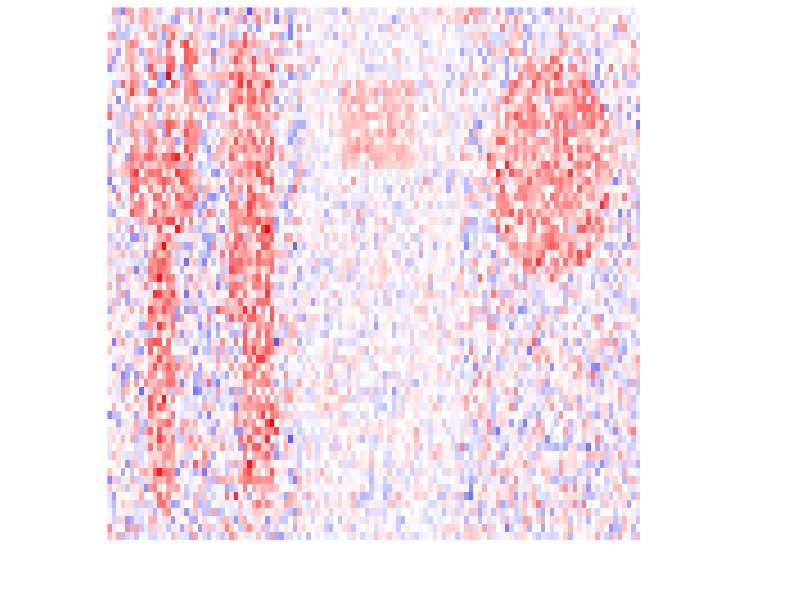
\includegraphics[width=0.35\textwidth]{images/heatmap_logistic_grp_simu_4000_bloc.png}} \\
        \subfloat[group lasso (variable)\label{fig:3000var}]{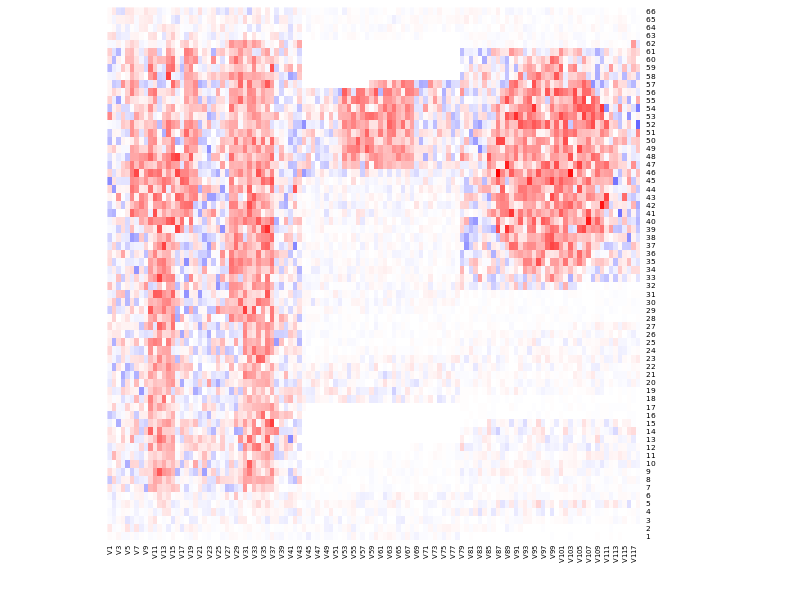
\includegraphics[width=0.35\textwidth]{images/heatmap_logistic_grp_simu_4000_var.png}} &
        \subfloat[group lasso (mode)\label{fig:3000mode}]{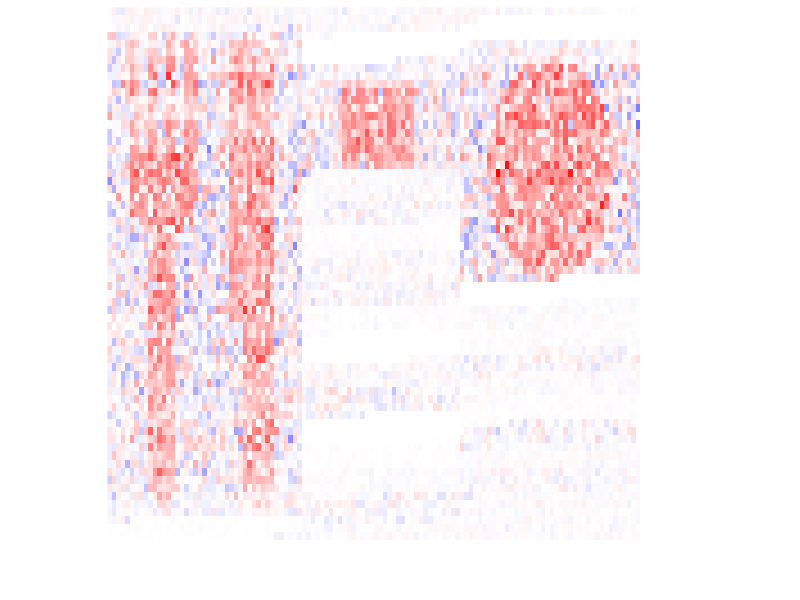
\includegraphics[width=0.35\textwidth]{images/heatmap_logistic_grp_simu_4000_mode.png}} \\
        \subfloat[multiway\label{fig:3000multiway}]{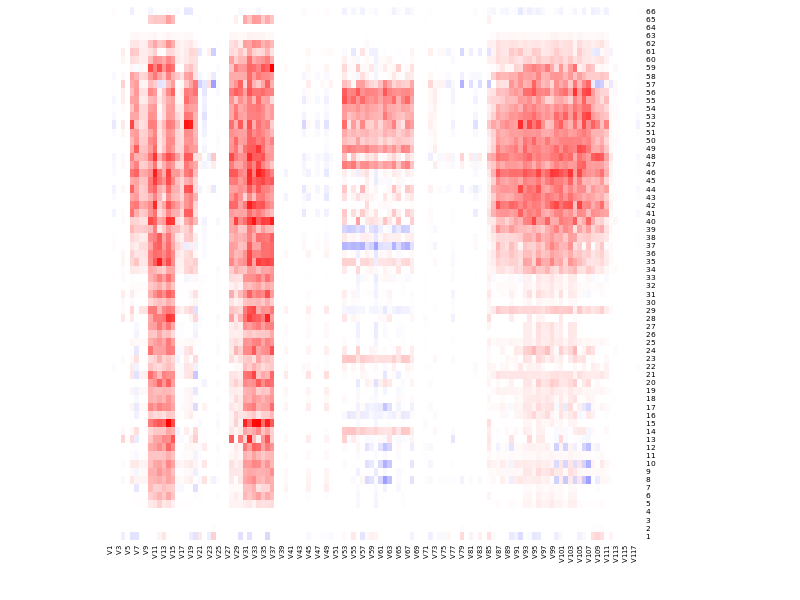
\includegraphics[width=0.35\textwidth]{images/heatmap_logistic_multibloc_simu_4000_multiway.png}} &
        \subfloat[multiway multibloc\label{fig:3000multibloc}]{
\includegraphics[width=0.35\textwidth]{images/heatmap_logistic_multibloc_simu_4000.png}} \\
    \end{tabular}
    \caption{Pictograms reconstructed by the different models for $3000$ individuals in the training dataset. The name of the model used is indicated in the legend of each figure.}
    \label{fig:tableau_figures_3000}
\end{figure}

\begin{figure}[H]
    \centering
    \begin{tabular}{cc}
        \subfloat[lasso \label{fig:500simple}]{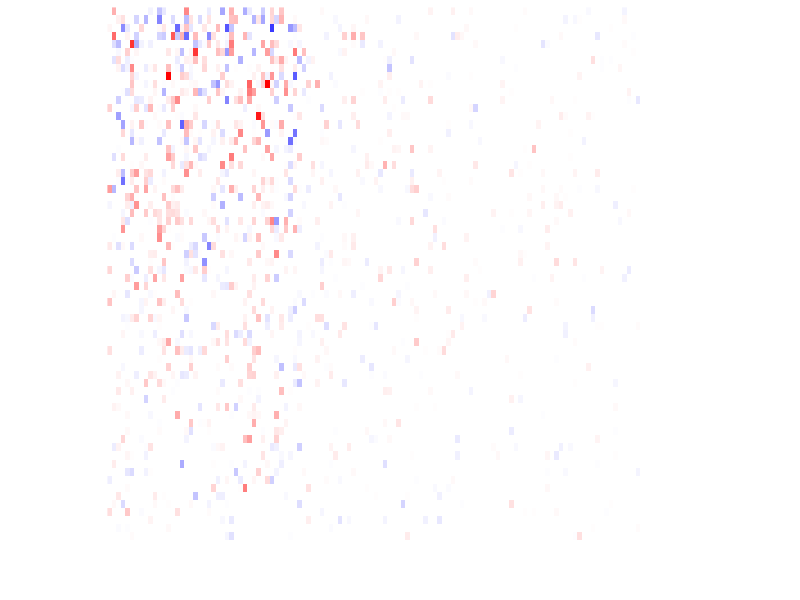
\includegraphics[width=0.35\textwidth]{images/picto_500/heatmap_logistique_simple_simu_500.png}} &
        \subfloat[group lasso (block)\label{fig:500bloc}]{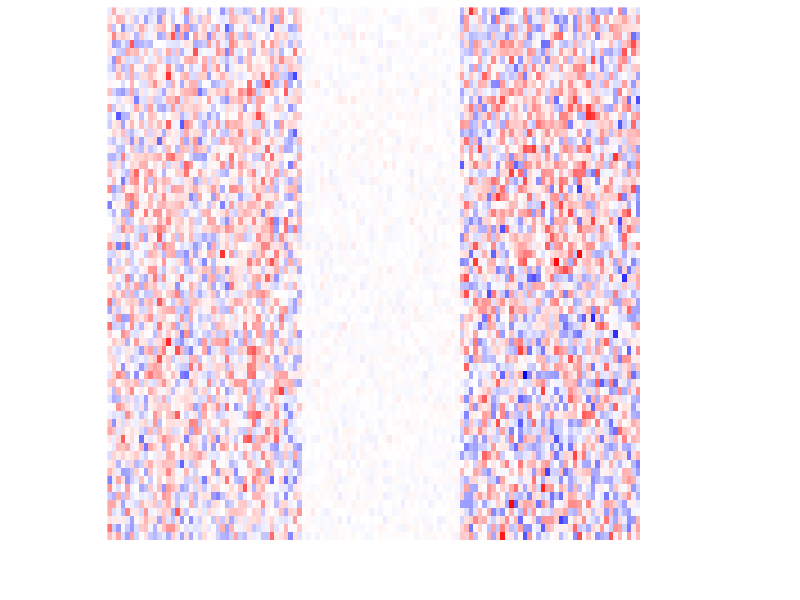
\includegraphics[width=0.35\textwidth]{images/picto_500/heatmap_logistic_grp_simu_500_bloc.png}} \\
        \subfloat[group lasso (variable)\label{fig:500var}]{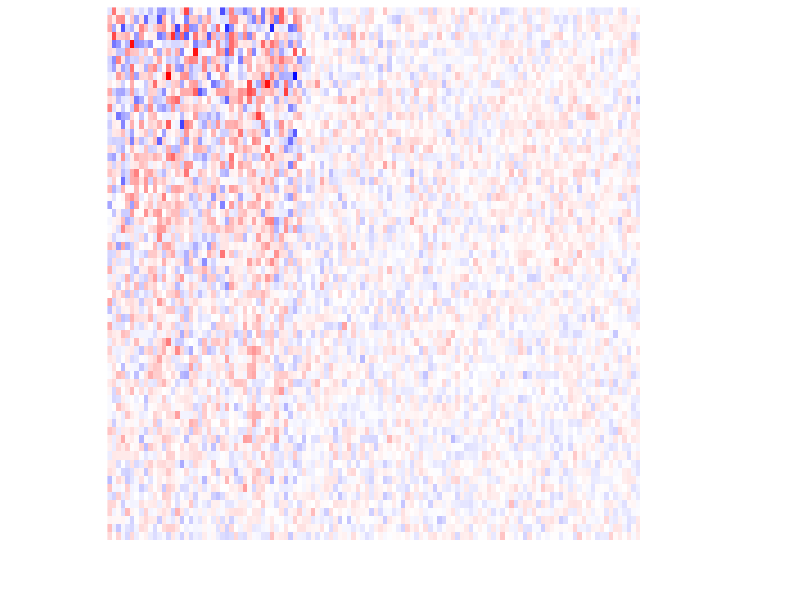
\includegraphics[width=0.35\textwidth]{images/picto_500/heatmap_logistic_grp_simu_500_var.png}} &
        \subfloat[group lasso (mode)\label{fig:500mode}]{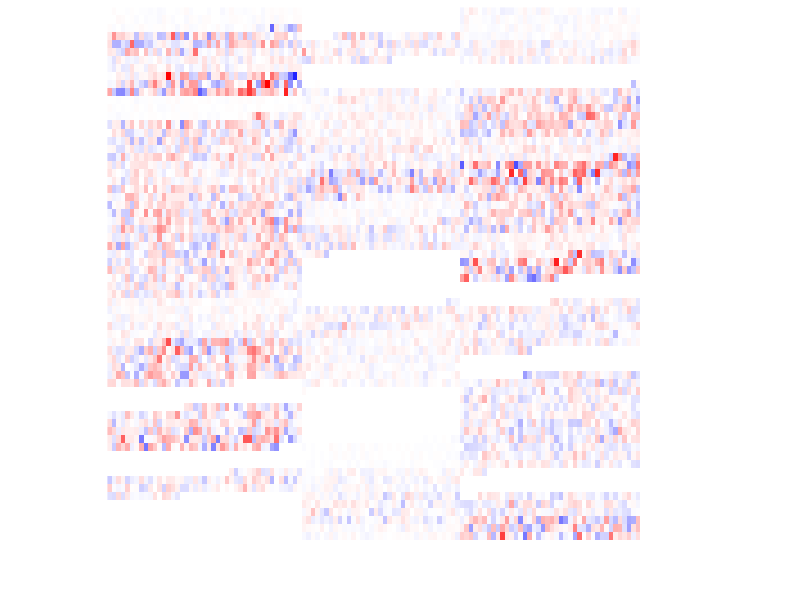
\includegraphics[width=0.35\textwidth]{images/picto_500/heatmap_logistic_grp_simu_500_mode.png}} \\
        \subfloat[multiway\label{fig:500multiway}]{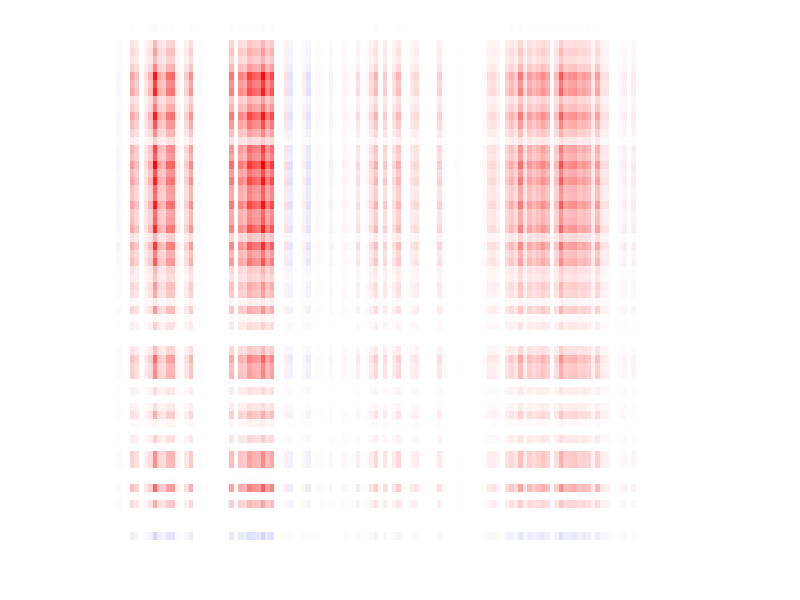
\includegraphics[width=0.35\textwidth]{images/picto_500/heatmap_logistic_multibloc_simu_500_multiway.png}} &
        \subfloat[multiway multibloc\label{fig:500multibloc}]{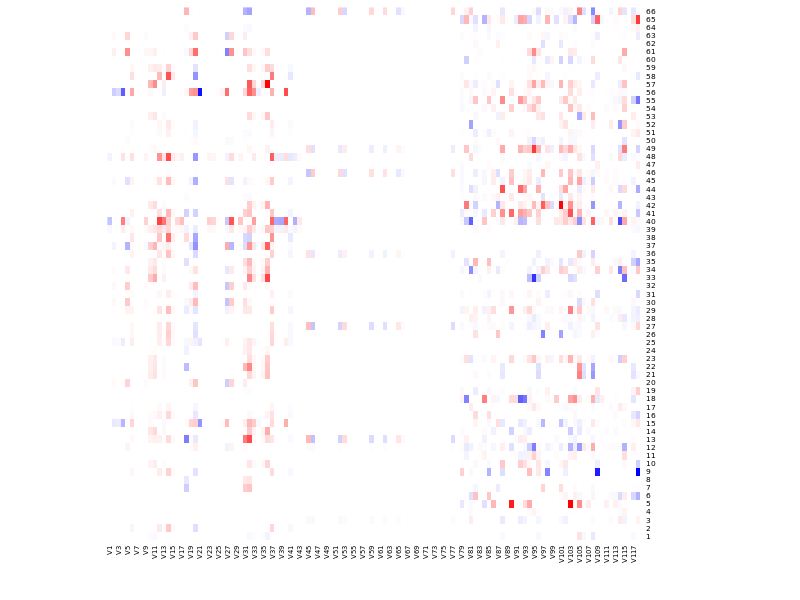
\includegraphics[width=0.35\textwidth]{images/picto_500/heatmap_logistic_multibloc_simu_500.png}} \\
    \end{tabular}
    \caption{Pictograms reconstructed by the different models for $500$ individuals in the training dataset. The name of the model used is indicated in the legend of each figure.}
    \label{fig:tableau_figures_500}
\end{figure}

\newpage 
\section{Importance of features}
\label{annexe:importance}
\noindent Importance graphs are given here for the best-performing models (in terms of AUC, see Table \ref{tab:result_real}), namely the group lasso model with block grouping for 3D data and the classic lasso for 2D data. The importance of a feature is measured as the absolute value of the $\beta$ coefficient in front of it. This value is then averaged over all simulations to find the feature's importance. Given the large number of features, we group them by block, mode and/or variable name. The importance of a group is given as the sum of the importances of its features. All group importances are finally renormalized so that their sum is $1$ (we're interested in the relative importance of features in relation to each other). \\
\indent On each stick of each bar chart, in addition to the importance, we can read a percentage in green. This provides information on the number of times the coefficient in front of the features associated with the stick has been non-zero in the simulations. As all our models are penalized by the lasso, they tend to set the coefficients of the least important variables to zero. We can therefore calculate for each variable, over the $50$ training sessions carried out, the percentage of times this coefficient was non-zero. The average of these percentages over all the features in a feature group (block, mode or variable) is shown in green on the graph. This average reflects the number of times the features in this group were deemed important by the model (i.e. their regression coefficient was non-zero).

\begin{figure}[H]
    \centering
    \begin{tabular}{cc}
        \subfloat[Relative importance of time on 3D data (excluding clinical data)\label{fig:3D_imp_time}]{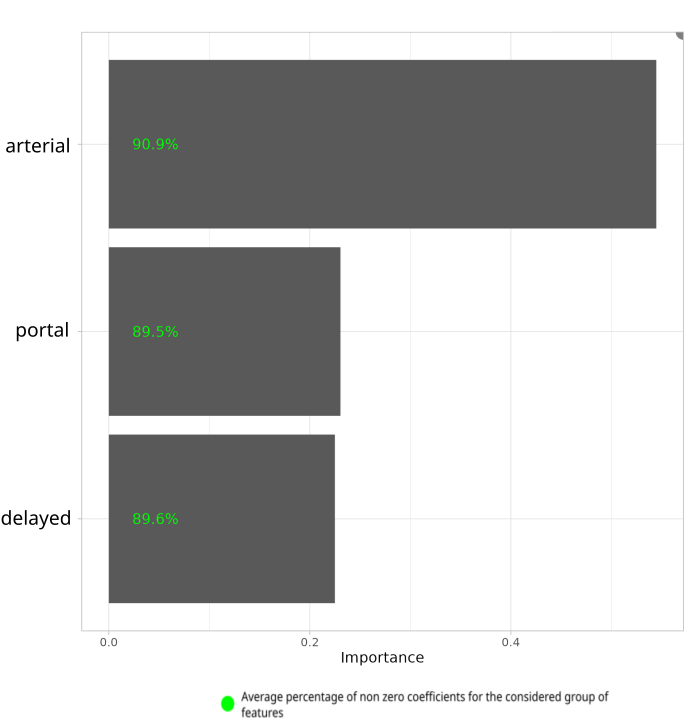
\includegraphics[width=0.45\textwidth]{images/importance/3D/global_big_groups_beta_valuereel_global_bloc.png}} &
        \subfloat[relative importance of blocks on 3D data\label{fig:3D_imp_bloc}]{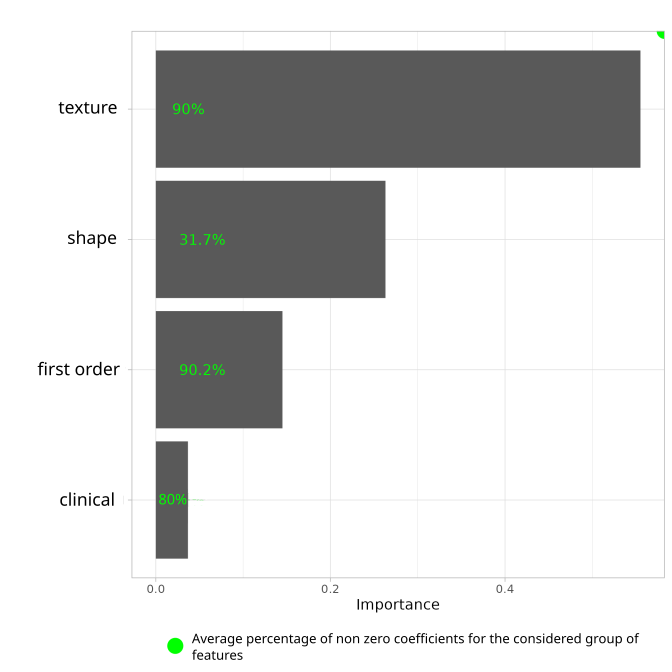
\includegraphics[width=0.45\textwidth]{images/importance/3D/global_blocs_beta_valuereel_global_bloc.png}} \\
    \end{tabular}
    \caption{Relative importance of features for 3D data with the best-performing model for this data: group lasso with block grouping (part 1)}
    \label{fig:imp_3D_1}
\end{figure}

\begin{figure}[H]
    \ContinuedFloat % Continuer la numérotation des sous-figures
    \centering
    \begin{tabular}{c}
        \subfloat[relative importance of block times on 3D data (excluding clinical data)\label{fig:3D_imp_bloc_and_mode}]{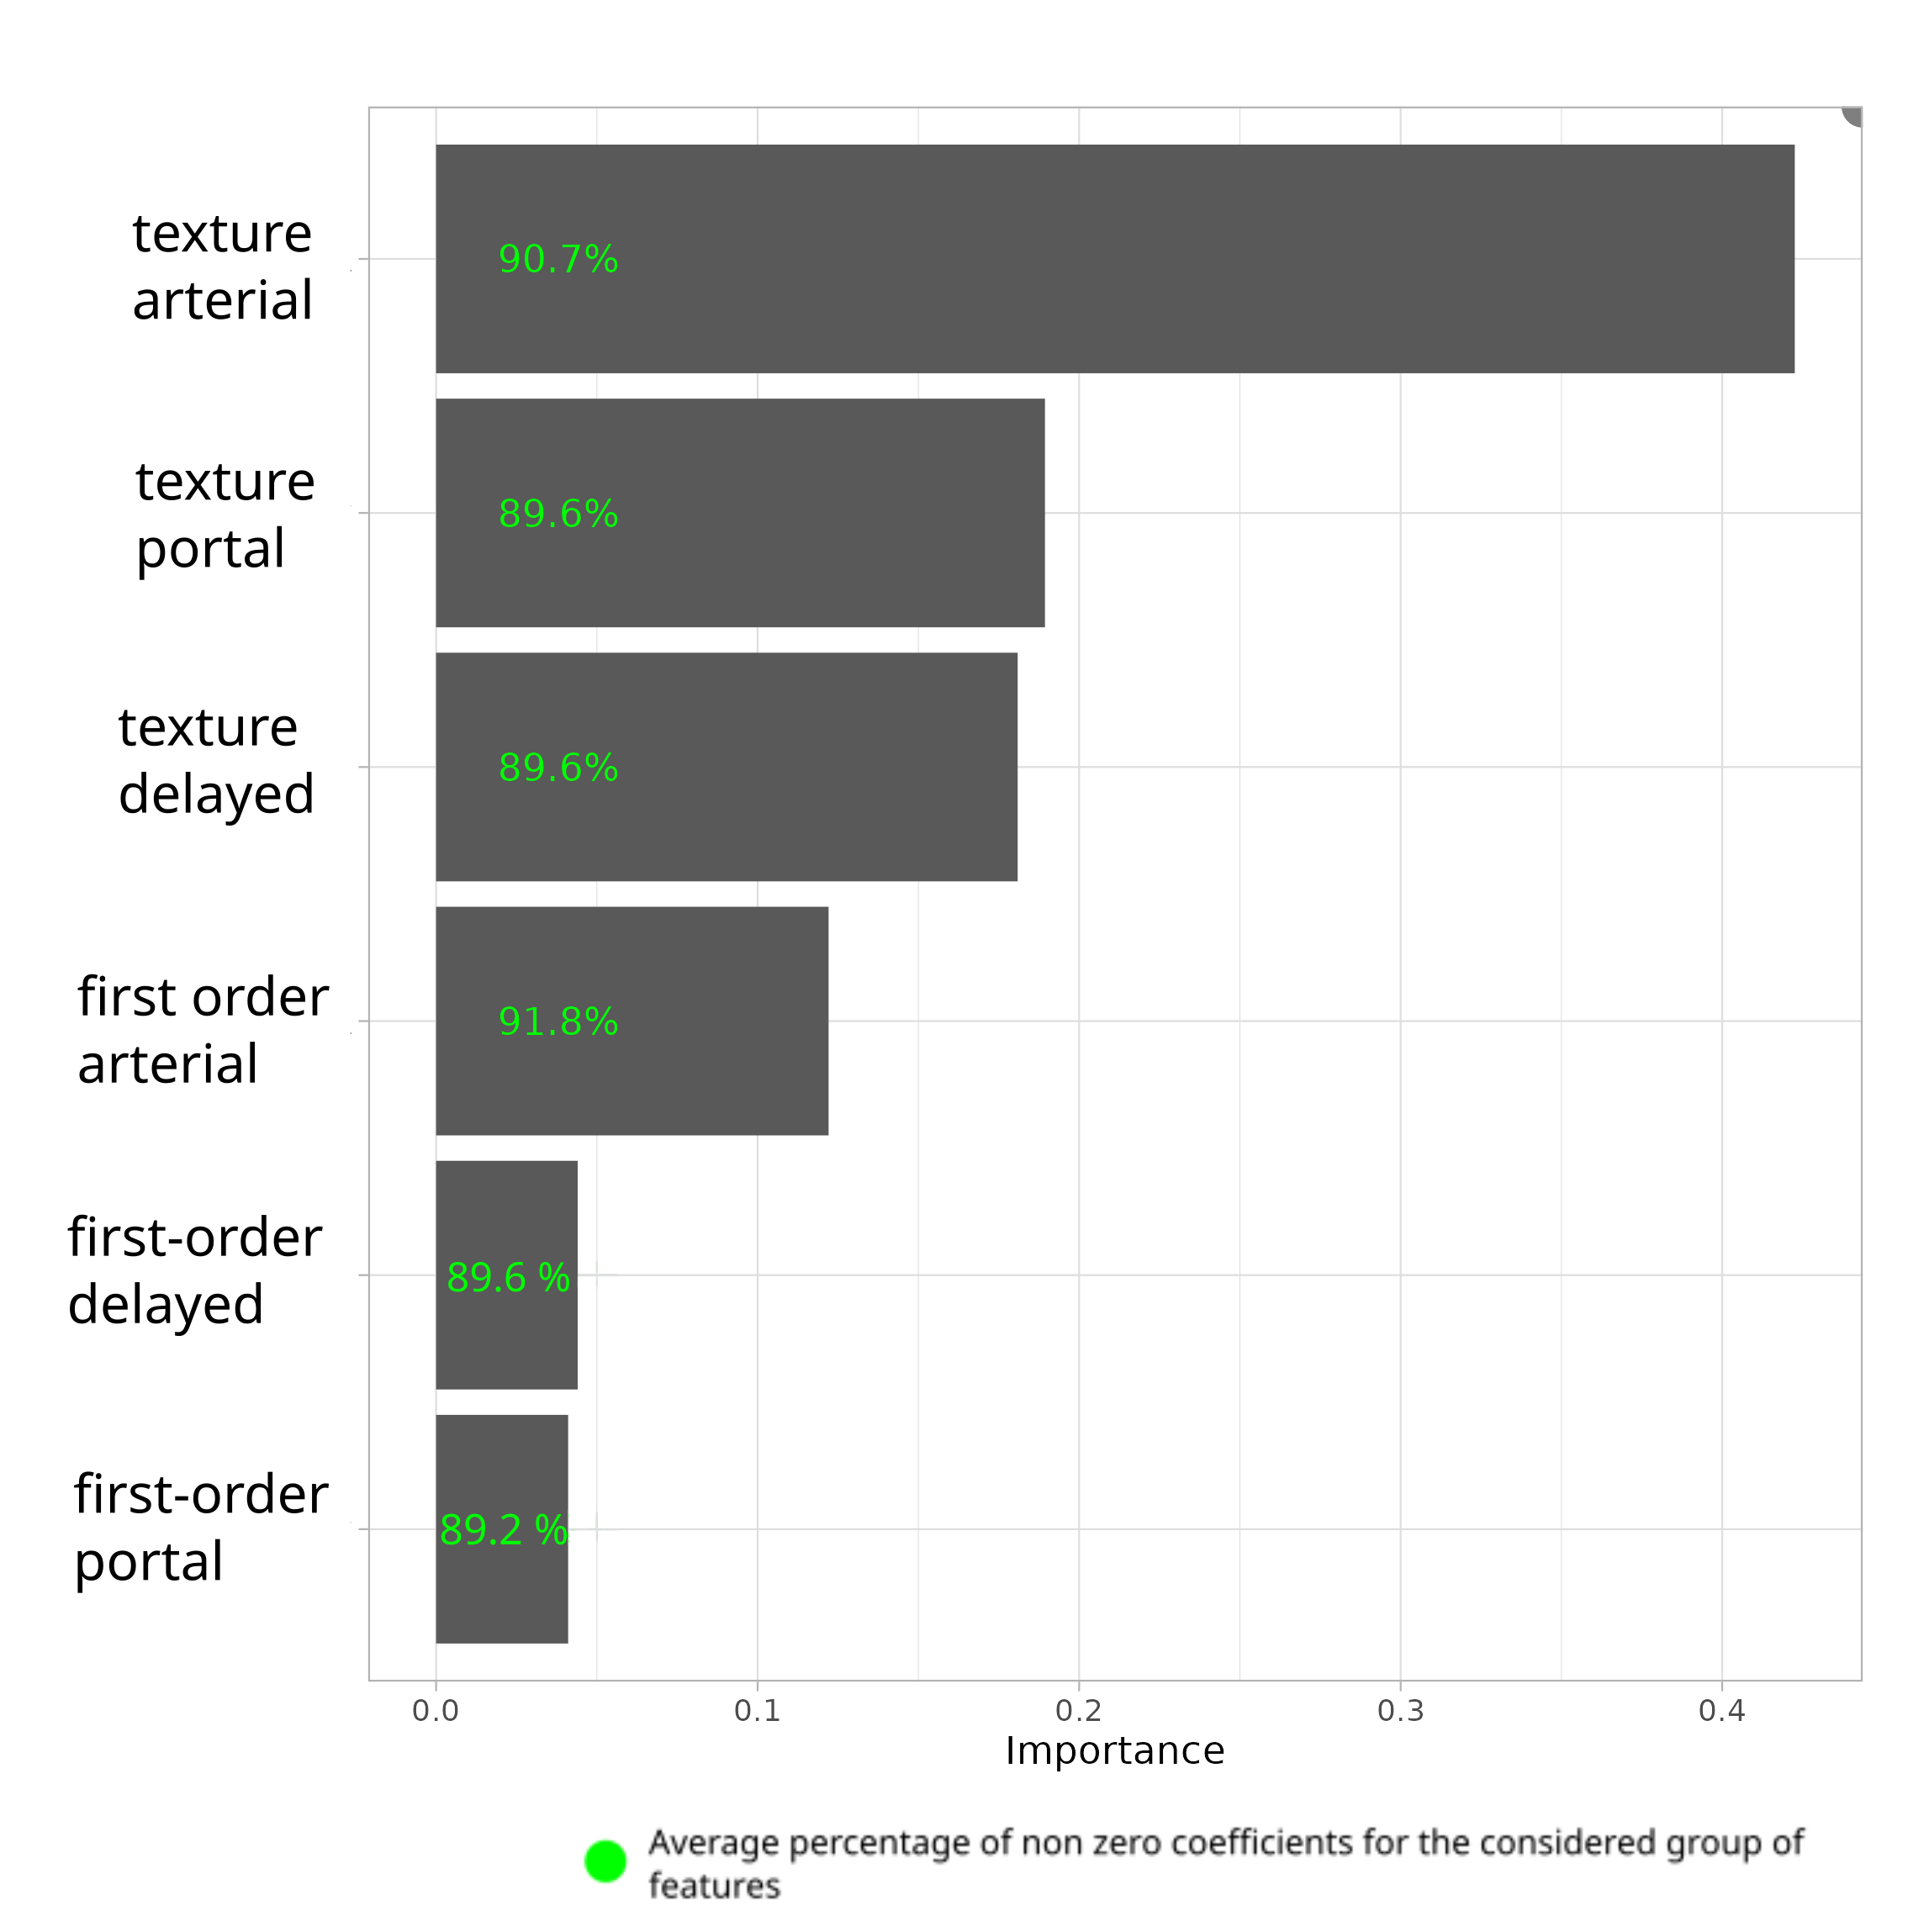
\includegraphics[width=0.5\textwidth]{images/importance/3D/global_bloc_and_mode_beta_valuereel_global_bloc.png}} 
    \end{tabular}
    \phantomcaption
    \label{fig:imp_3D_2}
\end{figure}

\vspace{0.2 cm}

\begin{figure}[H]
    \centering
    \begin{tabular}{cc}
        \subfloat[Relative importance of blocks on 2D data \label{fig:2D_imp_bloc}]{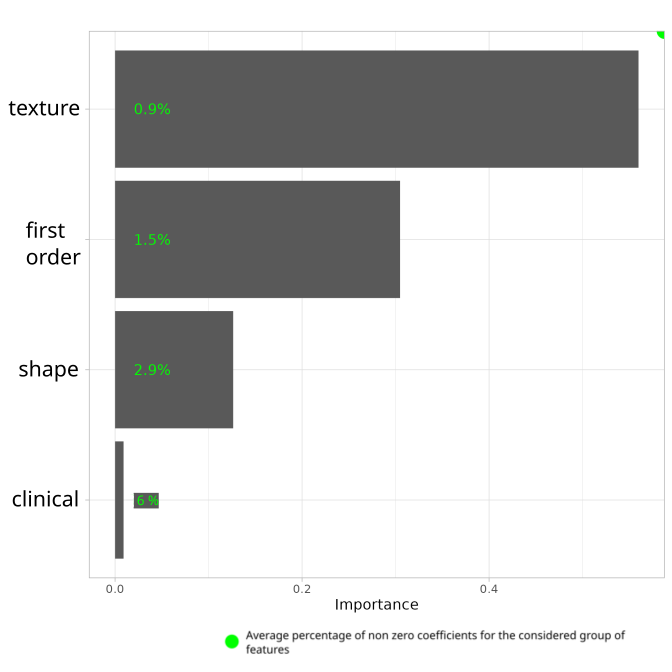
\includegraphics[width=0.45\textwidth]{images/importance/2D/global_blocs_beta_valuereel_multislice.png}} &
        \subfloat[relative importance of times per block on 2D data (excluding clinical data and shape featrues because they do not depend on time)\label{fig:2D_imp_bloc_time}]{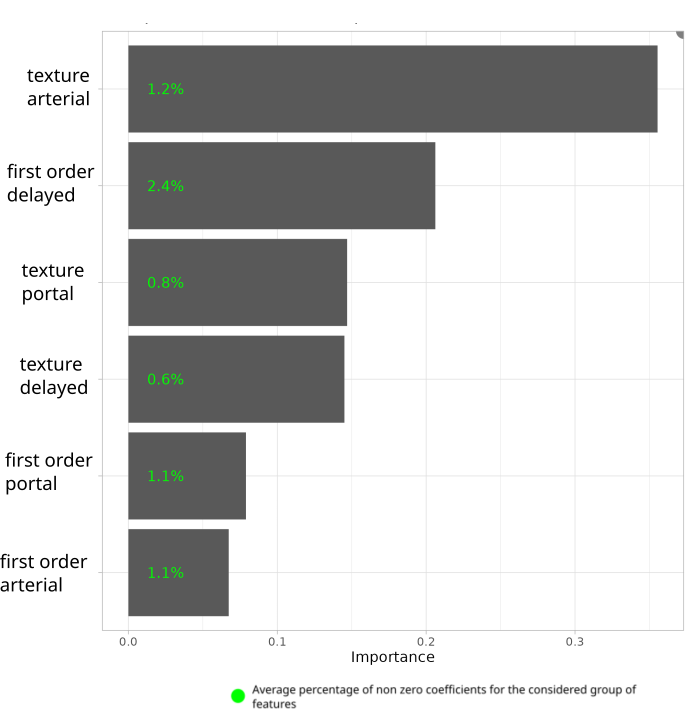
\includegraphics[width=0.45\textwidth]{images/importance/2D/global_mode_temps_beta_valuereel_multislice.png}} \\
    \end{tabular}
    \caption{Relative importance of features for 2D data with the best-performing model on these data: lasso logistic regression}
    \label{fig:imp_2D_1}
\end{figure}

\begin{figure}[H]
    \ContinuedFloat % Continuer la numérotation des sous-figures
    \centering
    \begin{tabular}{c}
        \subfloat[relative importance of slices per block on 2D data (excluding clinical data)\label{fig:2D_imp_bloc_slice}]{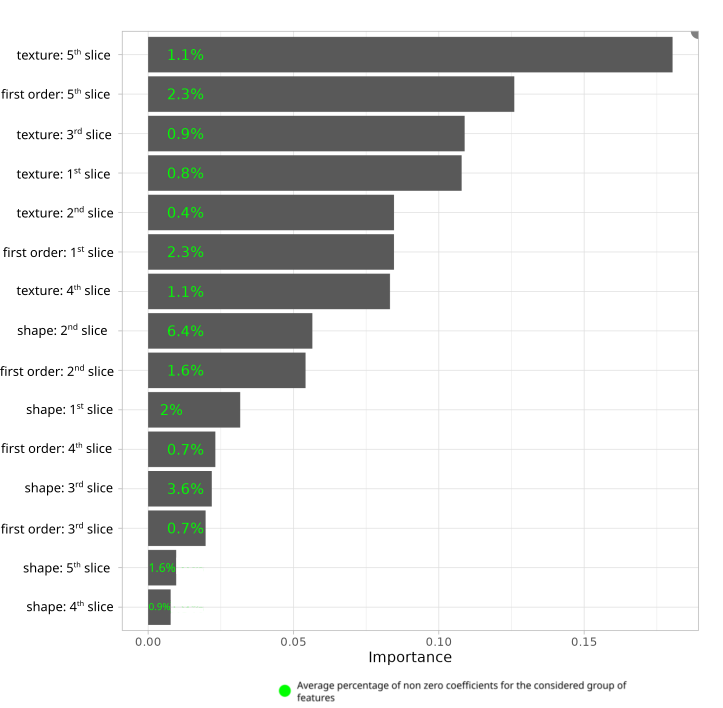
\includegraphics[width=0.5\textwidth]{images/importance/2D/global_mode_slice_beta_valuereel_multislice.png}} 
    \end{tabular}
    \phantomcaption
    \label{fig:imp_2D_2}
\end{figure}

\end{document}

\endinput
%%
%% End of file `elsarticle-template-num.tex'.
